\documentclass{report}

% Packages
\usepackage[utf8]{inputenc}
\usepackage[spanish]{babel}
\usepackage{amsmath}
\usepackage{amssymb}
\usepackage{amsthm}
\usepackage{graphicx}
\usepackage{float}
\usepackage{listings}
\usepackage{hyperref}
\usepackage[square,sort,comma,numbers]{natbib}
\usepackage{url}
\usepackage[strings]{underscore}

% All in preamble:

\usepackage{listings}
\usepackage{courier}
\usepackage{color}

\definecolor{mygreen}{rgb}{0,0.6,0}
\definecolor{mygray}{rgb}{0.5,0.5,0.5}
\definecolor{mymauve}{rgb}{0.58,0,0.82}
\lstset{ %
  backgroundcolor=\color{white},   % choose the background color; you must add \usepackage{color} or \usepackage{xcolor}
  basicstyle=\footnotesize\ttfamily,        % the size of the fonts that are used for the code
  breakatwhitespace=false,         % sets if automatic breaks should only happen at whitespace
  breaklines=true,                 % sets automatic line breaking
  captionpos=b,                    % sets the caption-position to bottom
  commentstyle=\color{mygreen},    % comment style
  deletekeywords={...},            % if you want to delete keywords from the given language
  escapeinside={\%*}{*)},          % if you want to add LaTeX within your code
  extendedchars=true,              % lets you use non-ASCII characters; for 8-bits encodings only, does not work with UTF-8
  frame=single,                    % adds a frame around the code
  keepspaces=true,                 % keeps spaces in text, useful for keeping indentation of code (possibly needs columns=flexible)
  keywordstyle=\color{blue},       % keyword style
  language=Python,                 % the language of the code
  otherkeywords={*,...},            % if you want to add more keywords to the set
  numbers=left,                    % where to put the line-numbers; possible values are (none, left, right)
  numbersep=5pt,                   % how far the line-numbers are from the code
  numberstyle=\tiny\color{mygray}, % the style that is used for the line-numbers
  rulecolor=\color{black},         % if not set, the frame-color may be changed on line-breaks within not-black text (e.g. comments (green here))
  showspaces=false,                % show spaces everywhere adding particular underscores; it overrides 'showstringspaces'
  showstringspaces=false,          % underline spaces within strings only
  showtabs=false,                  % show tabs within strings adding particular underscores
  stepnumber=2,                    % the step between two line-numbers. If it's 1, each line will be numbered
  stringstyle=\color{mymauve},     % string literal style
  tabsize=2,                       % sets default tabsize to 2 spaces
  title=\lstname                   % show the filename of files included with \lstinputlisting; also try caption instead of title
}

\hypersetup{
    colorlinks=true,
    linkcolor=blue,
    filecolor=magenta,      
    urlcolor=cyan,
    pdftitle={Overleaf Example},
    pdfpagemode=FullScreen,
}

\newtheorem{definition}{Definición}[section]
\newtheorem{theorem}{Teorema}
\newtheorem{lemma}{Lema}

\begin{document}

\begin{titlepage}
    \begin{center}
        \vspace*{1cm}
 
        \Large\textbf{Fractales}
 
        \vspace{0.5cm}
         Ejemplos, historia y aplicaciones
             
        \vspace{1.5cm}
 
        \textbf{Antonio Cabrera y Alejandro Gómez}
 
        \vfill
             
        Trabajo para el doble grado de\\
        Ingeniería del Software y Matemática Computacional\\
             
        \vspace{0.8cm}
      
        
\includegraphics[width=0.4\textwidth]{figures/logo u-tad.png}
             
        Asignatura de topología\\
        U-tad\\
        España\\
        Noviembre 2023
             
    \end{center}
 \end{titlepage}

\tableofcontents

\listoffigures

\chapter{Introducción}

\section{¿Qué es un fractal?}

La definición más inmediata que tenemos de los fractales es la siguiente:

\begin{definition}
    Un fractal es un objeto geométrico cuya estructura básica, fragmentada o irregular, se repite a diferentes escalas.
\end{definition}

\noindent Que su estructura básica se repita a diferentes escalas significa que el objeto es autosimilar.

\section{Autosimilitud}

Benoît Mandelbrot la definió como sigue:

\begin{definition}
    Un objeto es autosimilar o autosemejante si sus partes tienen la misma forma o estructura que el todo, aunque pueden presentarse a diferente escala y pueden estar ligeramente deformadas.
\end{definition}

\noindent
\large Vamos a ver dos tipos de autosimilitud:

\subsection{Autosimilitud exacta}

\begin{definition}
    Un objeto es exactamente autosimilar si es exactamente igual a sí mismo a diferentes escalas..
\end{definition}

\noindent
Es la más restrictiva de todas y la que vemos en los fractales clásicos. Algunos ejemplos de objetos exactamente autosimilares son:

\begin{itemize}
    \item El triángulo de Sierpinski
    
    \begin{figure}[H]
        \centering
        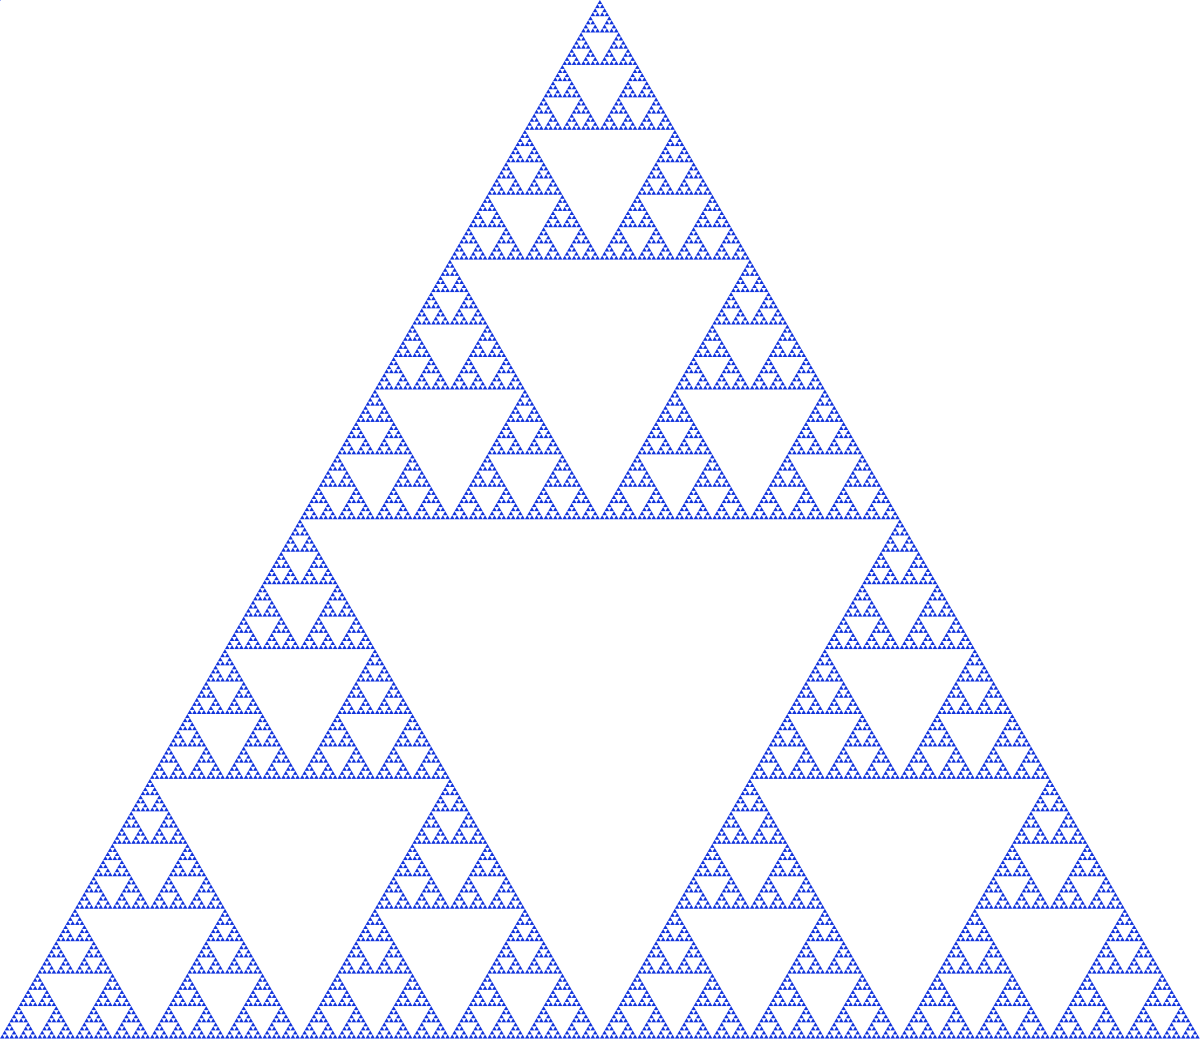
\includegraphics[width=0.5\textwidth]{figures/sierpinski-triangle.png}
        \caption{Triángulo de Sierpinski}
    \end{figure}

    \item El copo de Koch
    
    \begin{figure}[H]
        \centering
        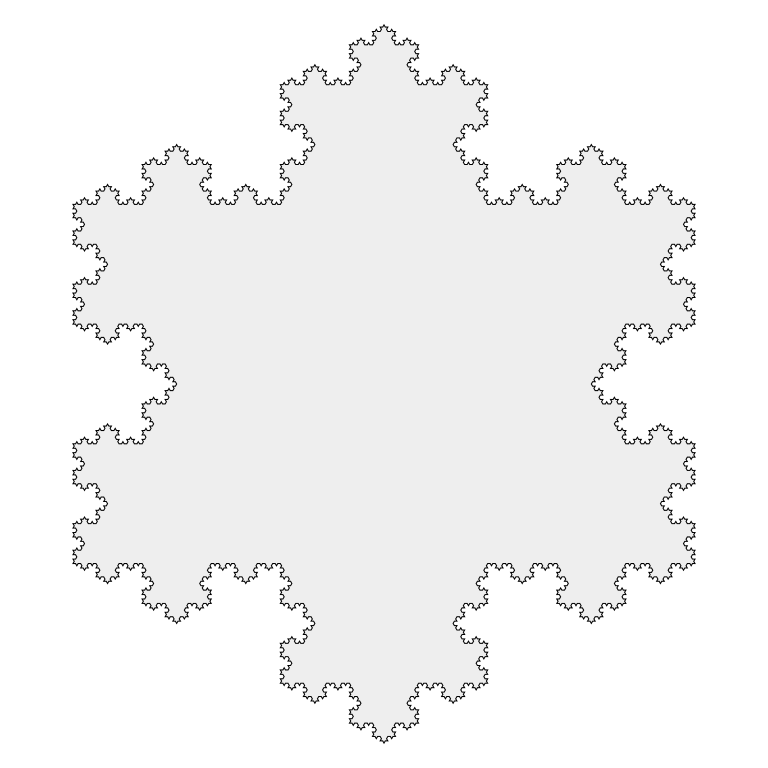
\includegraphics[width=0.5\textwidth]{figures/koch-snowflake.png}
        \caption{Copo de Koch}
    \end{figure}

\end{itemize}

\subsection{Cuasiautosimilitud}

\begin{definition}
    Un objeto es cuasiautosimilar si es aproximadamente igual a sí mismo a diferentes escalas.
\end{definition}

\noindent
Los fractales de este tipo contienen copias menores y distorsionadas de si mismos, como occure por ejemplo con el conjunto de Mandelbrot.

\begin{figure}[H]
    \centering
    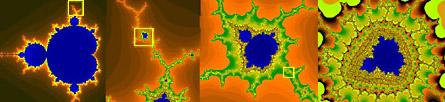
\includegraphics[width=0.7\textwidth]{figures/mandelbrot-cuasi.png}
    \caption{Ejemplos de cuasiautosimilitud en el conjunto de Mandelbrot}
\end{figure}


\section{Definición más formal}

\noindent En 1982 Benoît Mandelbrot definió los fractales de la siguiente forma:

\begin{definition}
Un fractal es un conjunto cuya dimensión de Hausdorff-Besicovitch es estrictamente mayor que su dimensión topológica.
\end{definition}

\noindent La dimensión topológica es la dimensión que todos conocemos, la dimensión de Hausdorff-Besicovitch es una de las formas de calcular la dimensión fractal de un objeto. 

\section{Dimensión fractal}

\noindent La dimensión fractal es una medida de la complejidad de un objeto fractal. La dimensión topológica de un objeto es un número entero, mientras que la dimensión fractal es un número real. La dimensión fractal es una generalización de la dimensión topológica.

\subsection{Cálculo de la dimensión fractal}

\noindent Ya hemos visto que una de las formas de calcular la dimensión fractal de un objeto es la dimensión de Hausdorff-Besicovitch, sin embargo esta resulta algo compleja. Otra forma más sencilla es con el método de \textit{Box Counting} también llamado o también conocido como la dimensión de Minkowski-Bouligard.\\

\noindent Para entender mejor este método vamos a verlo con un ejemplo. Consideremos un segemento y el borde de un cuadrado ambos de lado $1$.

\begin{figure}[H]
    \centering
    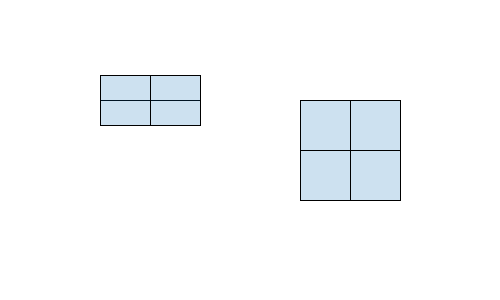
\includegraphics[width=0.7\textwidth]{figures/boxcounting-1.png}
    \caption{Box Counting - Cajas de lado $\frac{1}{2}$}
\end{figure}

\noindent Si intentamos cubrir ambos objetos con cajas de lado $\frac{1}{2}$ vemos que para el segmento necesitamos $2$ y para el cuadrado $2^2$

\begin{figure}[H]
    \centering
    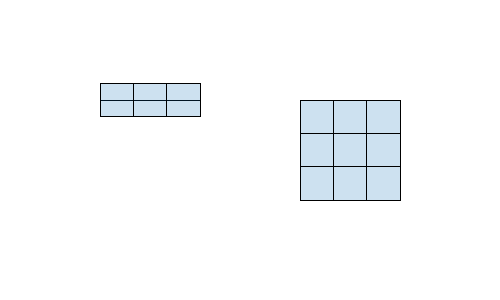
\includegraphics[width=0.7\textwidth]{figures/boxcounting-2.png}
    \caption{Box Counting - Cajas de lado $\frac{1}{3}$}
\end{figure}

\noindent Si utilizamos cajas más pequeñas, de lado $\frac{1}{3}$, vemos que para el segmento necesitamos $3$ y para el cuadrado $3^4$

\begin{figure}[H]
    \centering
    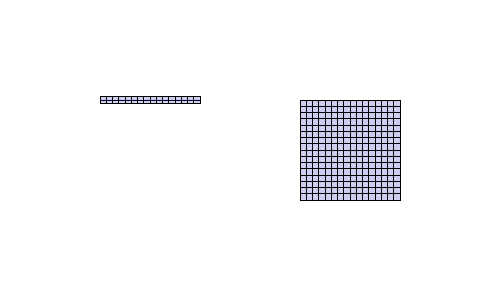
\includegraphics[width=0.7\textwidth]{figures/boxcounting-3.png}
    \caption{Box Counting - Cajas de lado $\frac{1}{n}$}
\end{figure}

\noindent Si continuamos con este proceso vemos que para el segmento necesitamos $n$ cajas de lado $\frac{1}{n}$ y para el cuadrado $n^2$\\

\noindent Vemos que el exponente es un buen indicador de la dimensión de los objetos. Si definimos $N(n)$ como el número de cajas de lado $\frac{1}{n}$ necesarias para cubrir el objeto, entonces tenemos que:

\begin{equation}
    N(n) = n^d
\end{equation}

\noindent Sacando logaritmos a ambos lados tenemos que:

\begin{equation}
    \log N(n) = \log n^d \Longleftrightarrow \log N(n) = d \log n \Longleftrightarrow d = \frac{\log N(n)}{\log n}
\end{equation}

\begin{definition}
    La dimensión de Minkowski-Bouligard de un conjunto $A$ es el límite de la expresión
    \begin{equation}
        \lim_{\epsilon \to 0} \frac{\log N(\epsilon)}{\log \frac{1}{\epsilon}}
    \end{equation}
    donde $N(\epsilon)$ es el mínimo de bolas de radio $\epsilon$ necesarias para recubrir el conjunto.
\end{definition}

\noindent Ahora vamos a ver que ocurre cuando intentamos calcular la dimensión de Minkowski-Bouligard de un fractal, como por ejemplo el triángulo de Sierpinski de base $1$.\\

\noindent Si intentamos cubrir el triángulo con cajas de lado $\frac{1}{2}$ vemos que necesitamos $4$ cajas.

\begin{figure}[H]
    \centering
    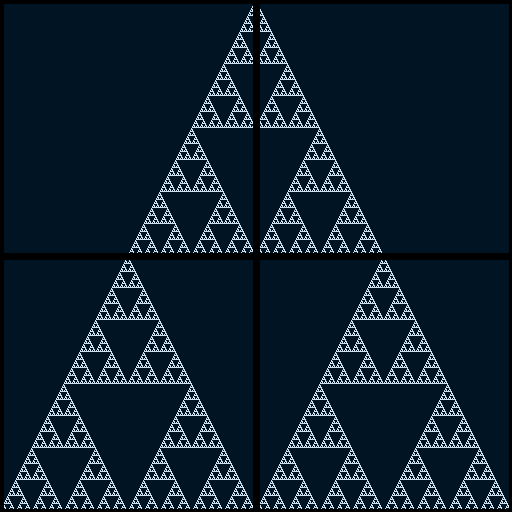
\includegraphics[width=0.5\textwidth]{figures/boxcounting-sierspinsky-1.png}
    \caption{Box Counting - Triángulo de Sierpinski - Cajas de lado $\frac{1}{2}$}
\end{figure}

\noindent Si utilizamos cajas más pequeñas, de lado $\frac{1}{4}$, necesitaremos $12$ cajas.

\begin{figure}[H]
    \centering
    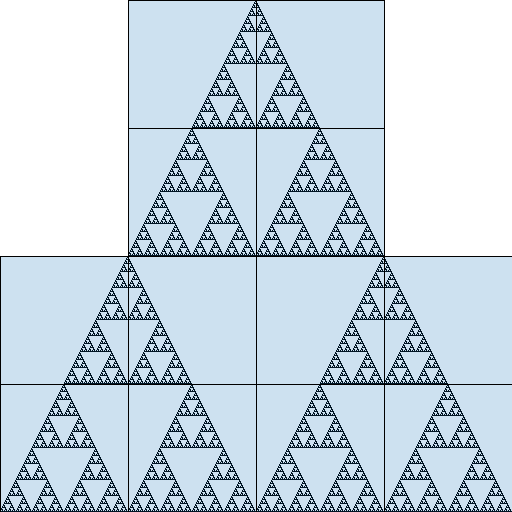
\includegraphics[width=0.5\textwidth]{figures/boxcounting-sierspinsky-2.png}
    \caption{Box Counting - Triángulo de Sierpinski - Cajas de lado $\frac{1}{4}$}
\end{figure}

\noindent Con cajas de lado $\frac{1}{8}$ necesitaremos $36$ cajas.

\begin{figure}[H]
    \centering
    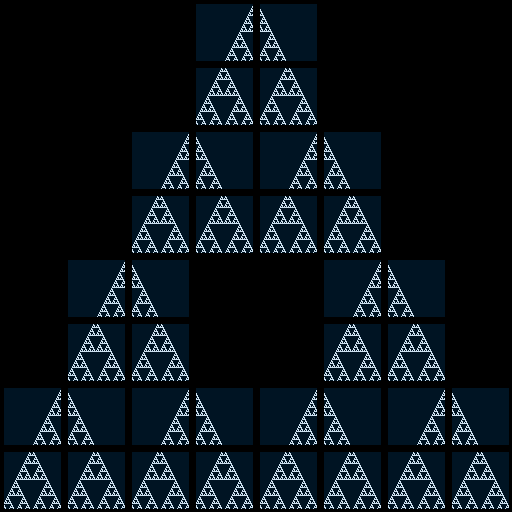
\includegraphics[width=0.5\textwidth]{figures/boxcounting-sierspinsky-3.png}
    \caption{Box Counting - Triángulo de Sierpinski - Cajas de lado $\frac{1}{8}$}
\end{figure}

\noindent Y con cajas de lado $\frac{1}{16}$ necesitaremos $108$ cajas.

\begin{figure}[H]
    \centering
    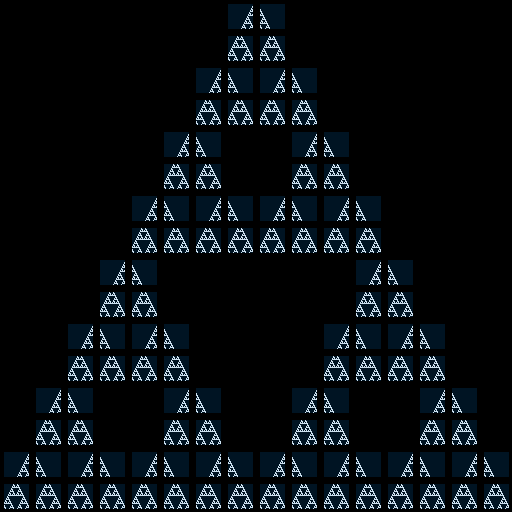
\includegraphics[width=0.5\textwidth]{figures/boxcounting-sierspinsky-4.png}
    \caption{Box Counting - Triángulo de Sierpinski - Cajas de lado $\frac{1}{16}$}
\end{figure}

\noindent Si continuamos con este proceso vemos que para el triángulo de Sierpinski necesitamos $4 \cdot 3^{n-1}$ cajas de lado $\frac{1}{2^n}$.
Si definimos $N(n)$ como el número de cajas de lado $\frac{1}{2^n}$ necesarias para cubrir el objeto, entonces tenemos que:

\begin{equation}
    \begin{split}
        & d = \lim_{n \rightarrow \infty} \frac{log (N(n))}{log (2^n)} = \lim_{n \rightarrow \infty} \frac{4 \cdot 3^{n-1}}{2^n} \approx \\
        & \approx \lim_{n \rightarrow \infty} \frac{3^n}{2^n} = \frac{\log{3}}{\log{2}} \approx 1.585\\
    \end{split}
\end{equation}

\noindent Como ya hemos comentado antes, nos sale un número real. Nuestra intuición nos sugiere que el triángulo de Sierpinski es \textit{"más que una curva"} pero \textit{"menos que una superficie"}\\


\chapter{Historia}

\section{Antecedentes}

\noindent Las primeras formas fractales aparecieron en el siglo XIX, cuando el matemático Karl Weierstrass graficó en 1872 su famosa función de Weierstrass. Más tarde en ese mismo siglo, empezaron a surgir conceptos cada vez más cercanos a lo que hoy se consideran fractales, siendo más gemométricos y menos algebraicos.\cite{complejidad}

\begin{figure}[H]
    \centering
    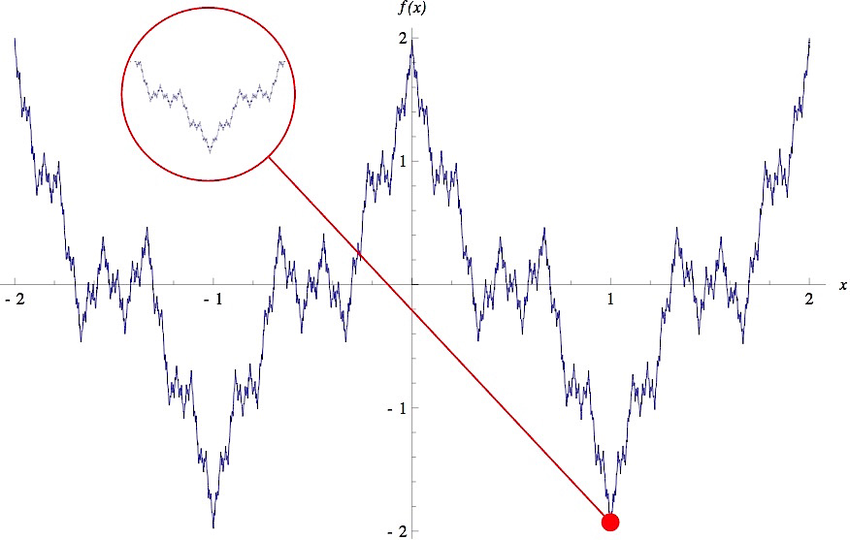
\includegraphics[width=0.5\textwidth]{figures/weierstrass-function.png}
    \caption{Función de Weierstrass}
    \label{fig:weierstrass-function}
\end{figure}

\section{Primeros fractales}

\noindent Así, en 1904, Helge von Koch definió su copo de nieve, una curva con propiedades similares a la de Weierstrass. En 1915, Waclaw Sierspinski construyó su triángulo y, un año después, su alfombra. \cite{complejidad}

\begin{figure}[H]
    \centering
    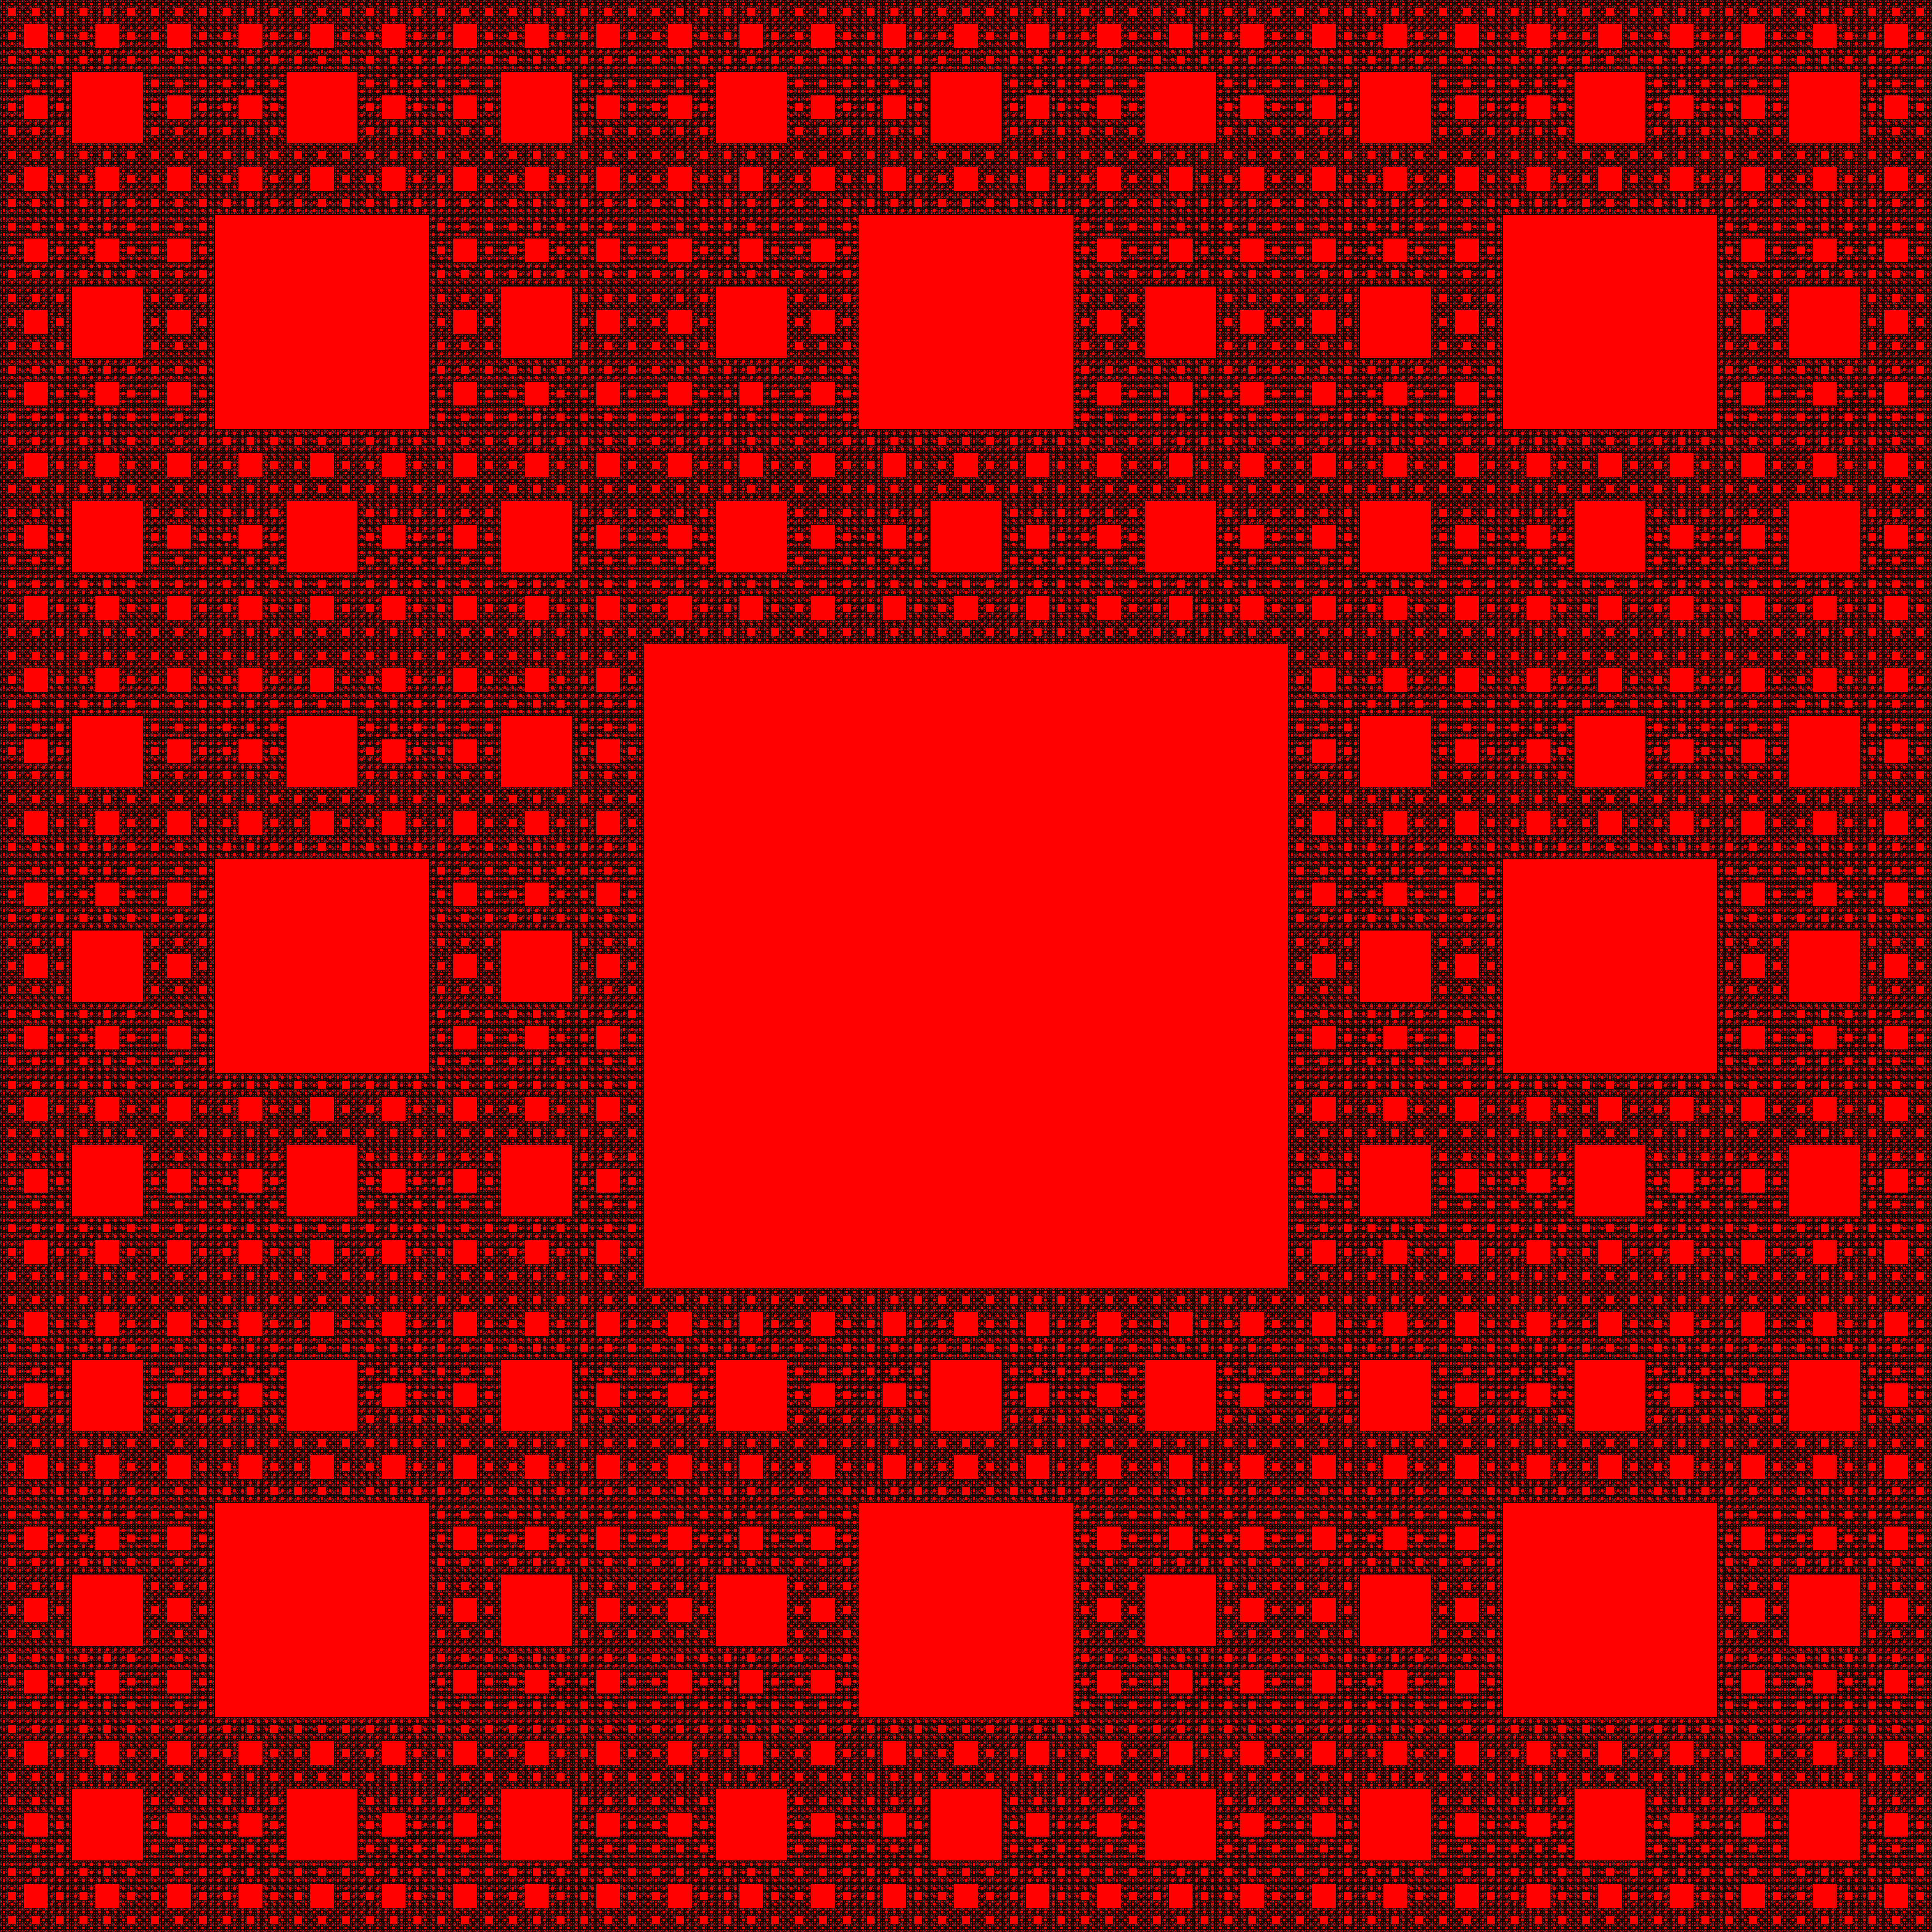
\includegraphics[width=0.5\textwidth]{figures/sierspinsky-carpet.png}
    \caption{Alfombra de Sierspinsky}
    \label{fig:sierspinsky-carpet}
\end{figure}

\section{Nuevas matemáticas}

\noindent En el siglo XIX, Georg Cantor desarrolló su conjunto de Cantor y 
Giuseppe Peano su curva de Peano. Gracias a esto se dieron cuenta de que estos objetos matemáticos no eran casos particulares, si no que había un gran conjunto de funciones que compartían las mismas cualidades que la función de Weierstrass. \cite{complejidad}\\ 

\begin{figure}[H]
    \centering
    
\includegraphics[width=0.5\textwidth]{figures/peano-curve.jpg}
    \caption{Curva de Peano}
    \label{fig:peano-curve}
\end{figure}


\noindent A pesar de que hubiese un gran conjunto de funciones, la geometría de Euclides y la dinámica Newtoniana no podían describirlas bien. En 1919, el matemático Félix Hausdorff introdujo la primera manera de observar y estudiar estos objetos, la dimensión de Hausdorff-Besicovitch. Años más tarde, Andrei Kolmogorov describió una herramienta similar conocida como la entropía de Kolmogorov. \cite{complejidad} \\

\noindent En 1963, Benoît Mandelbrot empezo a trabajar con los fractales a raíz de otra investigación, lo que le llevó a fundar la geometría fractal. \cite{complejidad}

\section{Mandelbrot}

\noindent Mandelbrot es uno de los mayores exponentes en el avance del campo de los fractales, desde identificar una muestra de \textit{"tiempo fractal"} hasta replantearse un problema mundialmente conocido: ¿Cuál es la longitud de la costa de Gran Bretaña? Según Mandelbrot esta distancia es infinita, o mejor dicho, depende de la longitud de la regla con la que se mida. Como ya hemos comentado, la geometría euclídea no es capaz de describir estos objetos, por lo que Mandelbrot utilizó la noción de dimensión, y en concreto, la extraña definición de dimensión fraccionarias. \cite{complejidad}\\

\noindent En 1975, Mandelbrot acuñó el término fractal, que proviene del latín \textit{fractus}, que significa roto o fracturado. El fractal más famoso de Mandelbrot es el conjunto de Mandelbrot, el cual es el más estudiado dentro del campo. \cite{complejidad}

\begin{figure}[H]
    \centering
    
\includegraphics[width=0.5\textwidth]{figures/mandelbrot-set-1.jpg}
    \caption{Conjunto de Mandelbrot}
    \label{fig:mandelbrot-set}
\end{figure}

\chapter{L-Systems}

\section{¿Qué son los L-Systems?}

\noindent Un sistema-L o también denominados sistemas de Lindenmayer se trata de un conjunto de reglas y símbolos usados para modelar el proceso de crecimiento de las plantas.

\noindent Fueron introducidos en 1968 por Aristid Lindenmayer, el cual estudió los patrones de crecimiento de varias algas y tenían como objetivo realizar una descripción formal del desarrollo de organismos y representar la relación entre células de plantas.

\section{¿Cómo funcionan?}

\noindent Las reglas de estos sistemas se basa en la autosimilitud, por eso las figuras que se suelen modelar suelen representar formas de tipo fractal.

\noindent Los sistemas-L se definen como un conjunto $G=\{V,S, \omega ,P\}$

\begin{itemize}
    \item $V$ es un conjunto de símbolos que contiene elementos que pueden ser reemplazados.
    \item $S$ es un conjunto de símbolos que contiene elementos que se mantienen fijos.
    \item $\omega$ es una cadena de símbolos de $V$ que definen el estado inicial del sistema (inicio o axioma).
    \item $P$ es un conjunto de reglas o producciones que definen la forma en la que las variables pueden ser reemplazadas por combinaciones de constantes y otras variables.
\end{itemize}

\noindent Todos los sistemas-L parten de un estado inicial, y se dice que el sistema es libre de contexto si cada iteración se refiere sólo a un símbolo individual y no a sus vecinos. Cuando la aplicación de una regla depende también de sus vecinos, se dice que el sistema-L es sensitivo al contexto.

\section{Ejemplos}

\subsection{Algas}

\noindent Pongamos como ejemplo de sistema-L el primer caso que quiso estudiar Lindenmayer, las algas.

\noindent Datos:

\begin{itemize}
    \item Variables: $A,B$
    \item Constantes: ninguna
    \item Incio: $A$
    \item Reglas: $A \rightarrow AB, B \rightarrow A$
\end{itemize}

\noindent Resultado:

\begin{itemize}
    \item Iteración 0: $A$
    \item Iteración 1: $AB$
    \item Iteración 2: $ABA$
    \item Iteración 3: $ABAAB$
    \item Iteración 4: $ABAABABA$
    \item Iteración 5: $ABAABABAABAAB$
\end{itemize}

\subsection{Copos de nieve}

\noindent Los sistemas también pueden ser representado con dibujos, el siguiente ejemplo se refiere a la variante de la curva de Koch con ángulo de 90:\\

\noindent Sintaxis:

\begin{equation}
    \begin{split}
        & F\rightarrow \text{Dibujar hacia adelante}\\
        & +\rightarrow \text{Girar a la izquierda } 90 \text{ grados}\\
        & -\rightarrow \text{Girar a la derecha } 90 \text{ grados}\\
    \end{split}
\end{equation}

\noindent Datos:

\begin{itemize}
    \item Variables: $F$
    \item Constantes: $+,-$
    \item Incio: $F$
    \item Reglas: $F \rightarrow F+F-F-F+F$
\end{itemize}

\noindent Resultado:\\

\noindent Para $n=0$ tenemos $F$:

\begin{figure}[H]
    
    \centering
    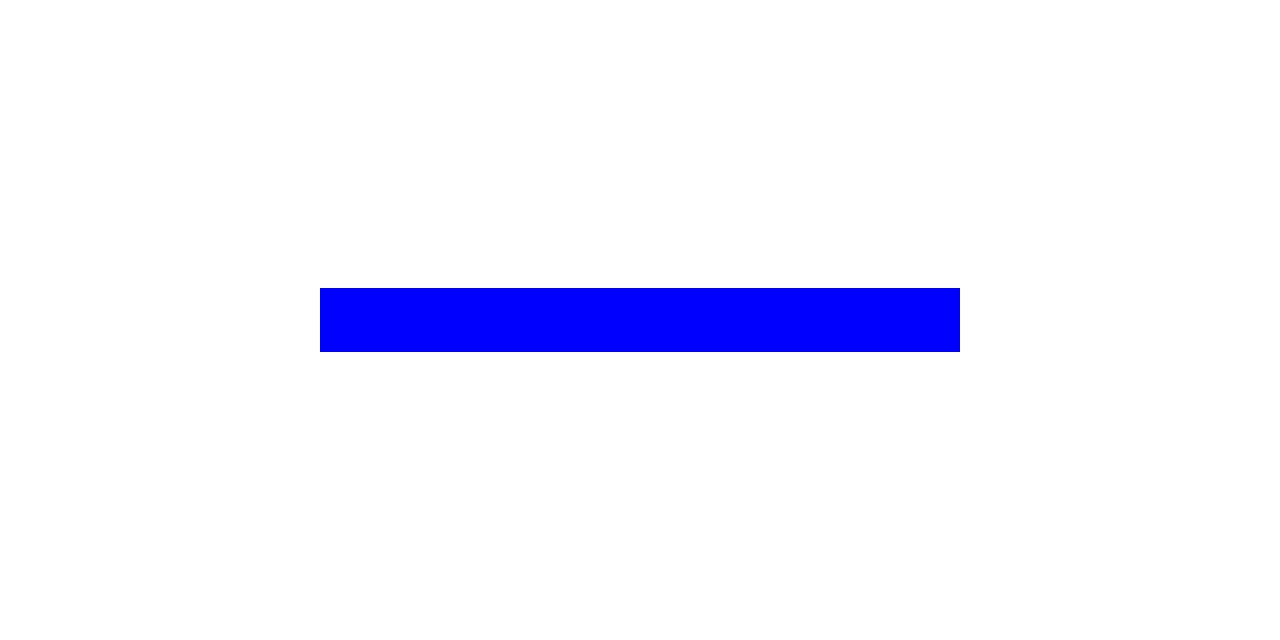
\includegraphics[width=0.5\textwidth]{figures/l-system-kock-snowflake-1.png}
    \caption{Curva de Koch con ángulo de 90 grados - 0 iteraciones}
    \label{fig:koch-snowflake-1}
\end{figure}

\noindent Para $n=1$ tenemos $F+F-F-F+F$:

\begin{figure}[H]
    \centering
    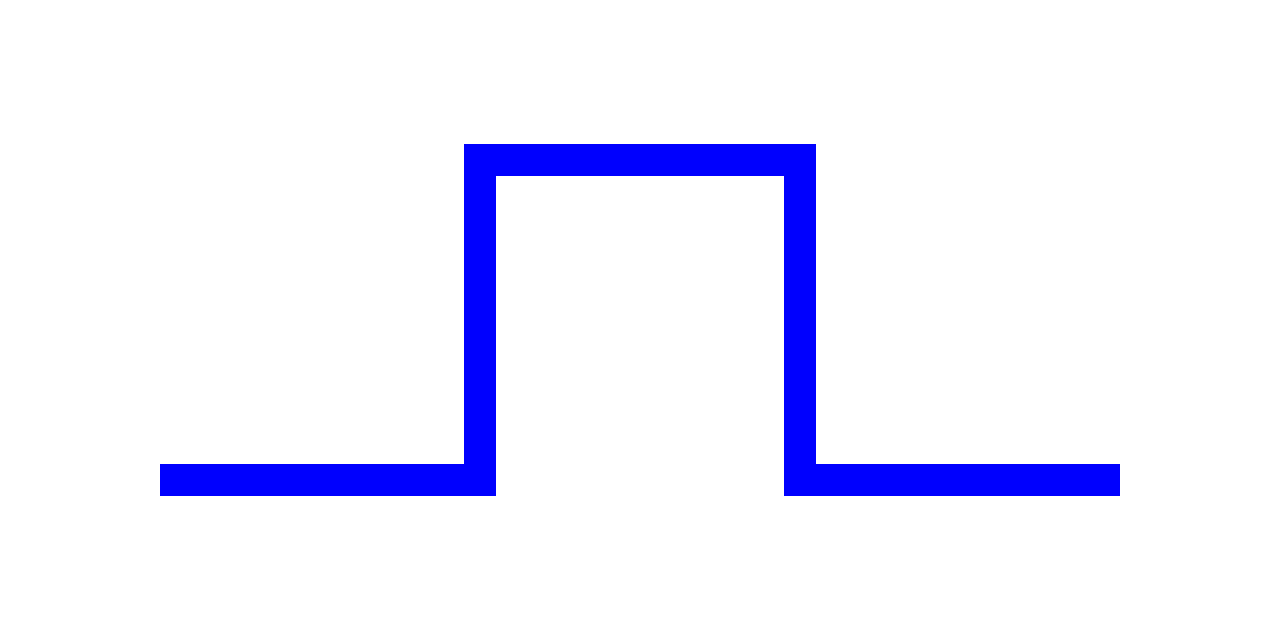
\includegraphics[width=0.5\textwidth]{figures/l-system-kock-snowflake-2.png}
    \caption{Curva de Koch con ángulo de 90 grados - 1 iteración}
    \label{fig:koch-snowflake-2}
\end{figure}

\noindent Para $n=2$ tenemos $F+F-F-F+F+F+F-F-F+F-F+F-F-F+F-F+F-F-F+F+F+F-F-F+F$:

\begin{figure}[H]
    \centering
    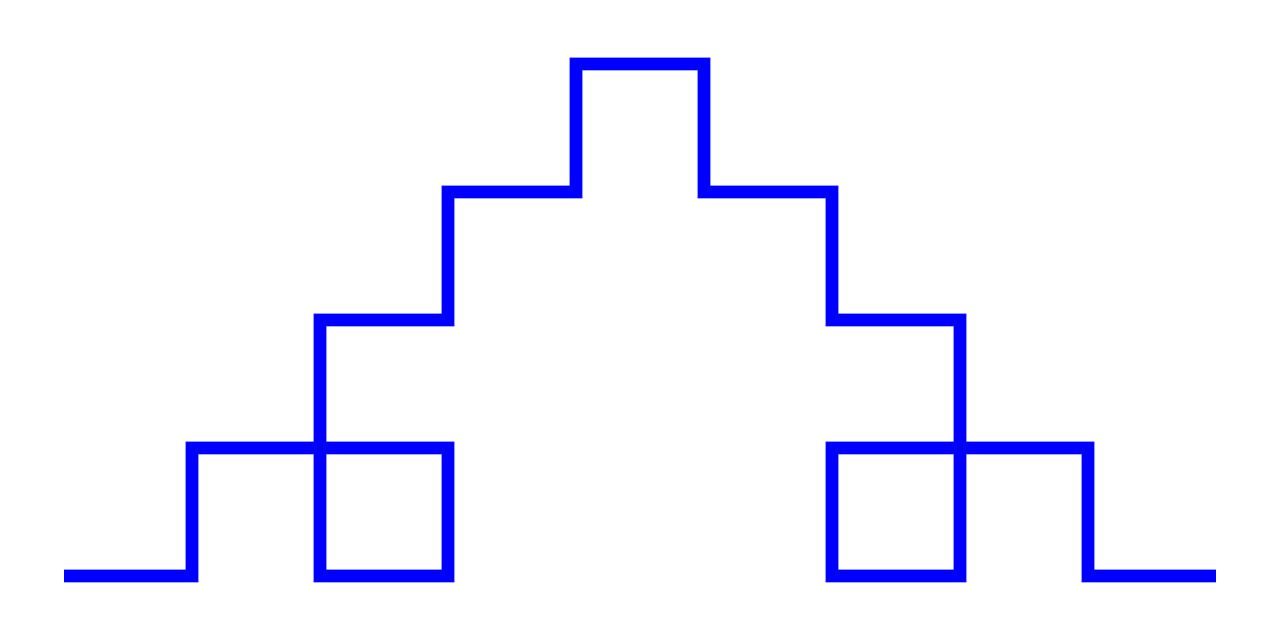
\includegraphics[width=0.5\textwidth]{figures/l-system-kock-snowflake-3.png}
    \caption{Curva de Koch con ángulo de 90 grados - 2 iteraciones}
    \label{fig:koch-snowflake-3}
\end{figure}

\noindent Para $n=3$ la secuencia es demasiado larga para ponerla aquí, pero el resultado es el siguiente:

\begin{figure}[H]
    \centering
    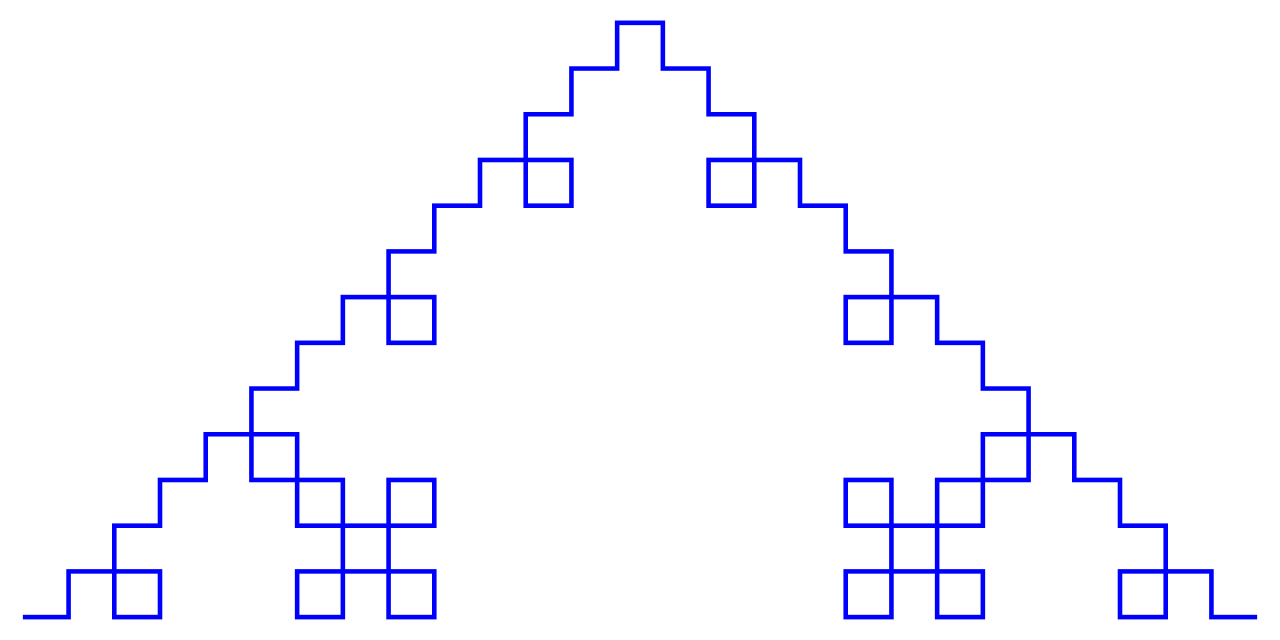
\includegraphics[width=0.5\textwidth]{figures/l-system-kock-snowflake-4.png}
    \caption{Curva de Koch con ángulo de 90 grados - 3 iteraciones}
    \label{fig:koch-snowflake-4}
\end{figure}

\section{Dibujos de plantas con L-Systems}

\subsection{Planta 1}

\begin{figure}[H]
    \centering
    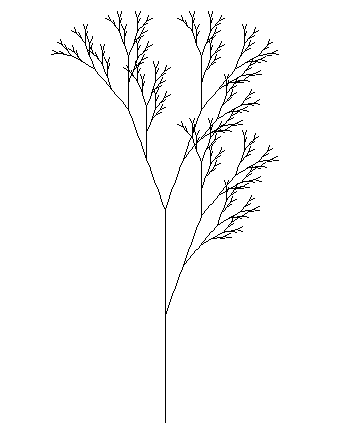
\includegraphics[width=0.5\textwidth]{figures/l-system-plant-1.png}
    \caption{Planta 1}
    \label{fig:plant-1}
    \cite{web-2023}
\end{figure}

\subsection{Planta 2}

\begin{figure}[H]
    \centering
    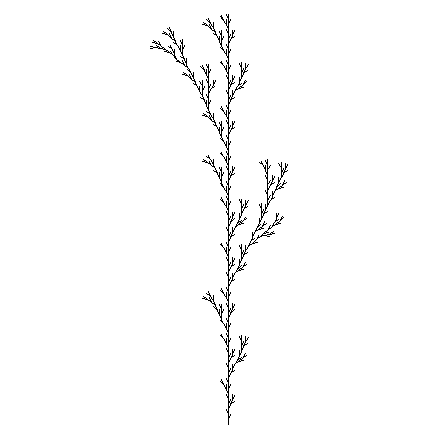
\includegraphics[width=0.5\textwidth]{figures/l-system-plant-2.png}
    \caption{Planta 2}
    \label{fig:plant-2}
    \cite{web-2023}
\end{figure}

\subsection{Planta 3}

\begin{figure}[H]
    \centering
    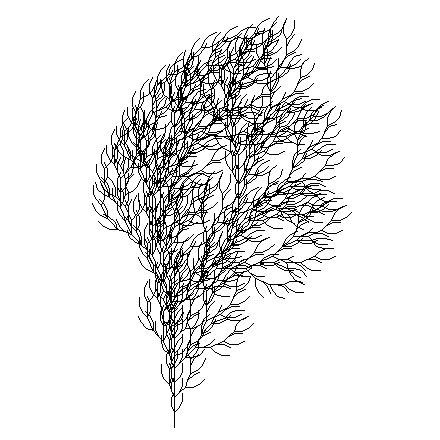
\includegraphics[width=0.5\textwidth]{figures/l-system-plant-3.png}
    \caption{Planta 3}
    \label{fig:plant-3}
    \cite{web-2023}
\end{figure}

\chapter{Ejemplos de fractales}

\section{Copo de Koch}

\subsection{Construcción}

\noindent Comenzamos con un segmento de longitud $1$.

\begin{figure}[H]
    \centering
    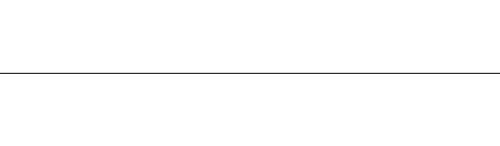
\includegraphics[width=0.5\textwidth]{figures/kock-curve-iteration-0.png}
    \caption{Iteración cero de la curva de Koch.}
    \label{fig:koch-curve-iteration-0}
\end{figure}

\noindent En la primera iteración, dividimos el segmento en tres partes iguales y reemplazamos la parte central por dos segmentos de la misma longitud, formando un ángulo de $60^\circ$. \cite{eswiki:copo-koch}

\begin{figure}[H]
    \centering
    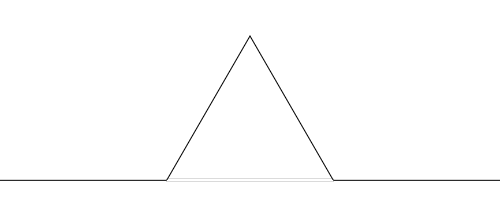
\includegraphics[width=0.5\textwidth]{figures/kock-curve-iteration-1.png}
    \caption{Primera iteración de la curva de Koch.}
    \label{fig:koch-curve-iteration-1}
\end{figure}

\noindent Para siguientes iteraciones, repetimos el mismo proceso para todos los segmentos. \cite{eswiki:copo-koch}

\begin{figure}[H]
    \centering
    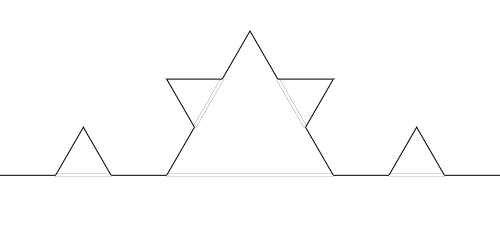
\includegraphics[width=0.5\textwidth]{figures/kock-curve-iteration-2.png}
    \caption{Segunda iteración de la curva de Koch.}
    \label{fig:koch-curve-iteration-2}
\end{figure}

\subsection{Propiedades}

\noindent El copo de Kock es un objeto autosimilar, con autosimilitud exacta. \cite{youtube-2022}

\begin{figure}[H]
\centering
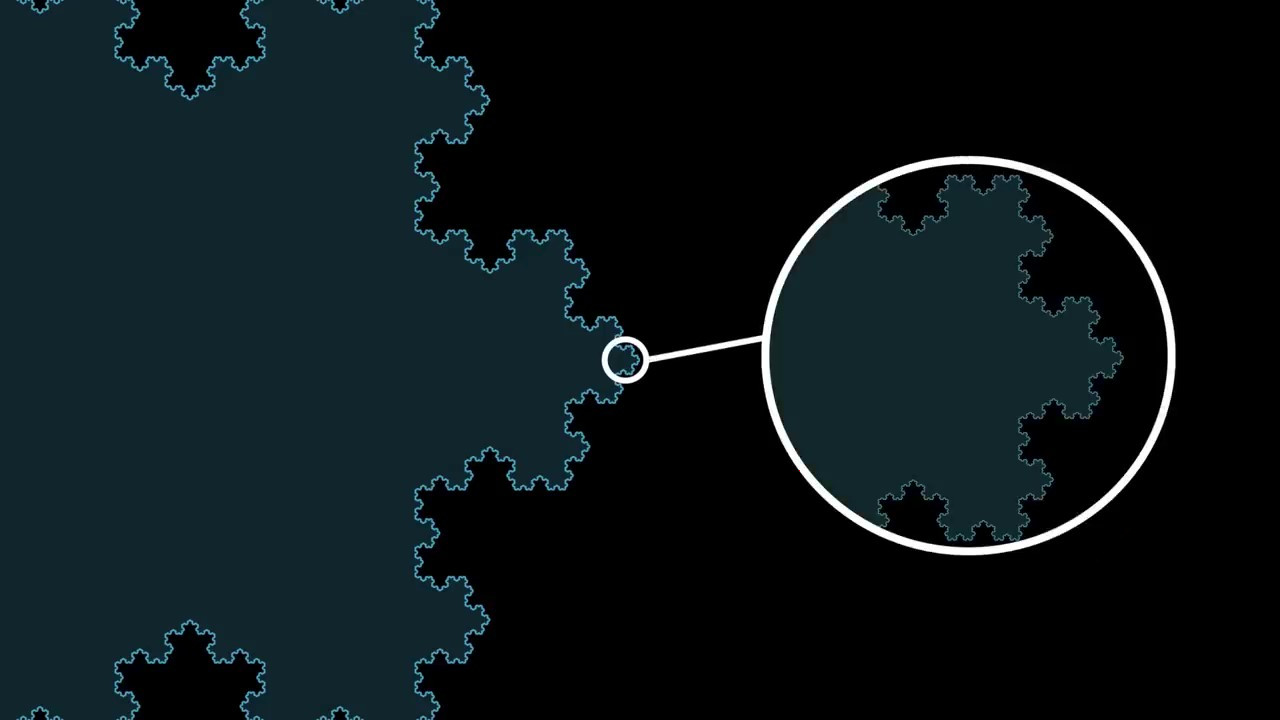
\includegraphics[width=0.5\textwidth]{figures/kock-snowflake-self-similarity.jpg}
\caption{Autosilitud exacta del copo de Koch.}
\label{fig:koch-snowflake-self-similarity}
\cite{youtube-2022}
\end{figure}

\noindent La dimensión fractal del copo de Koch es $\frac{\log 4}{\log 3} \approx 1.26186$ \cite{eswiki:copo-koch}\\

\begin{figure}[H]
    \centering
    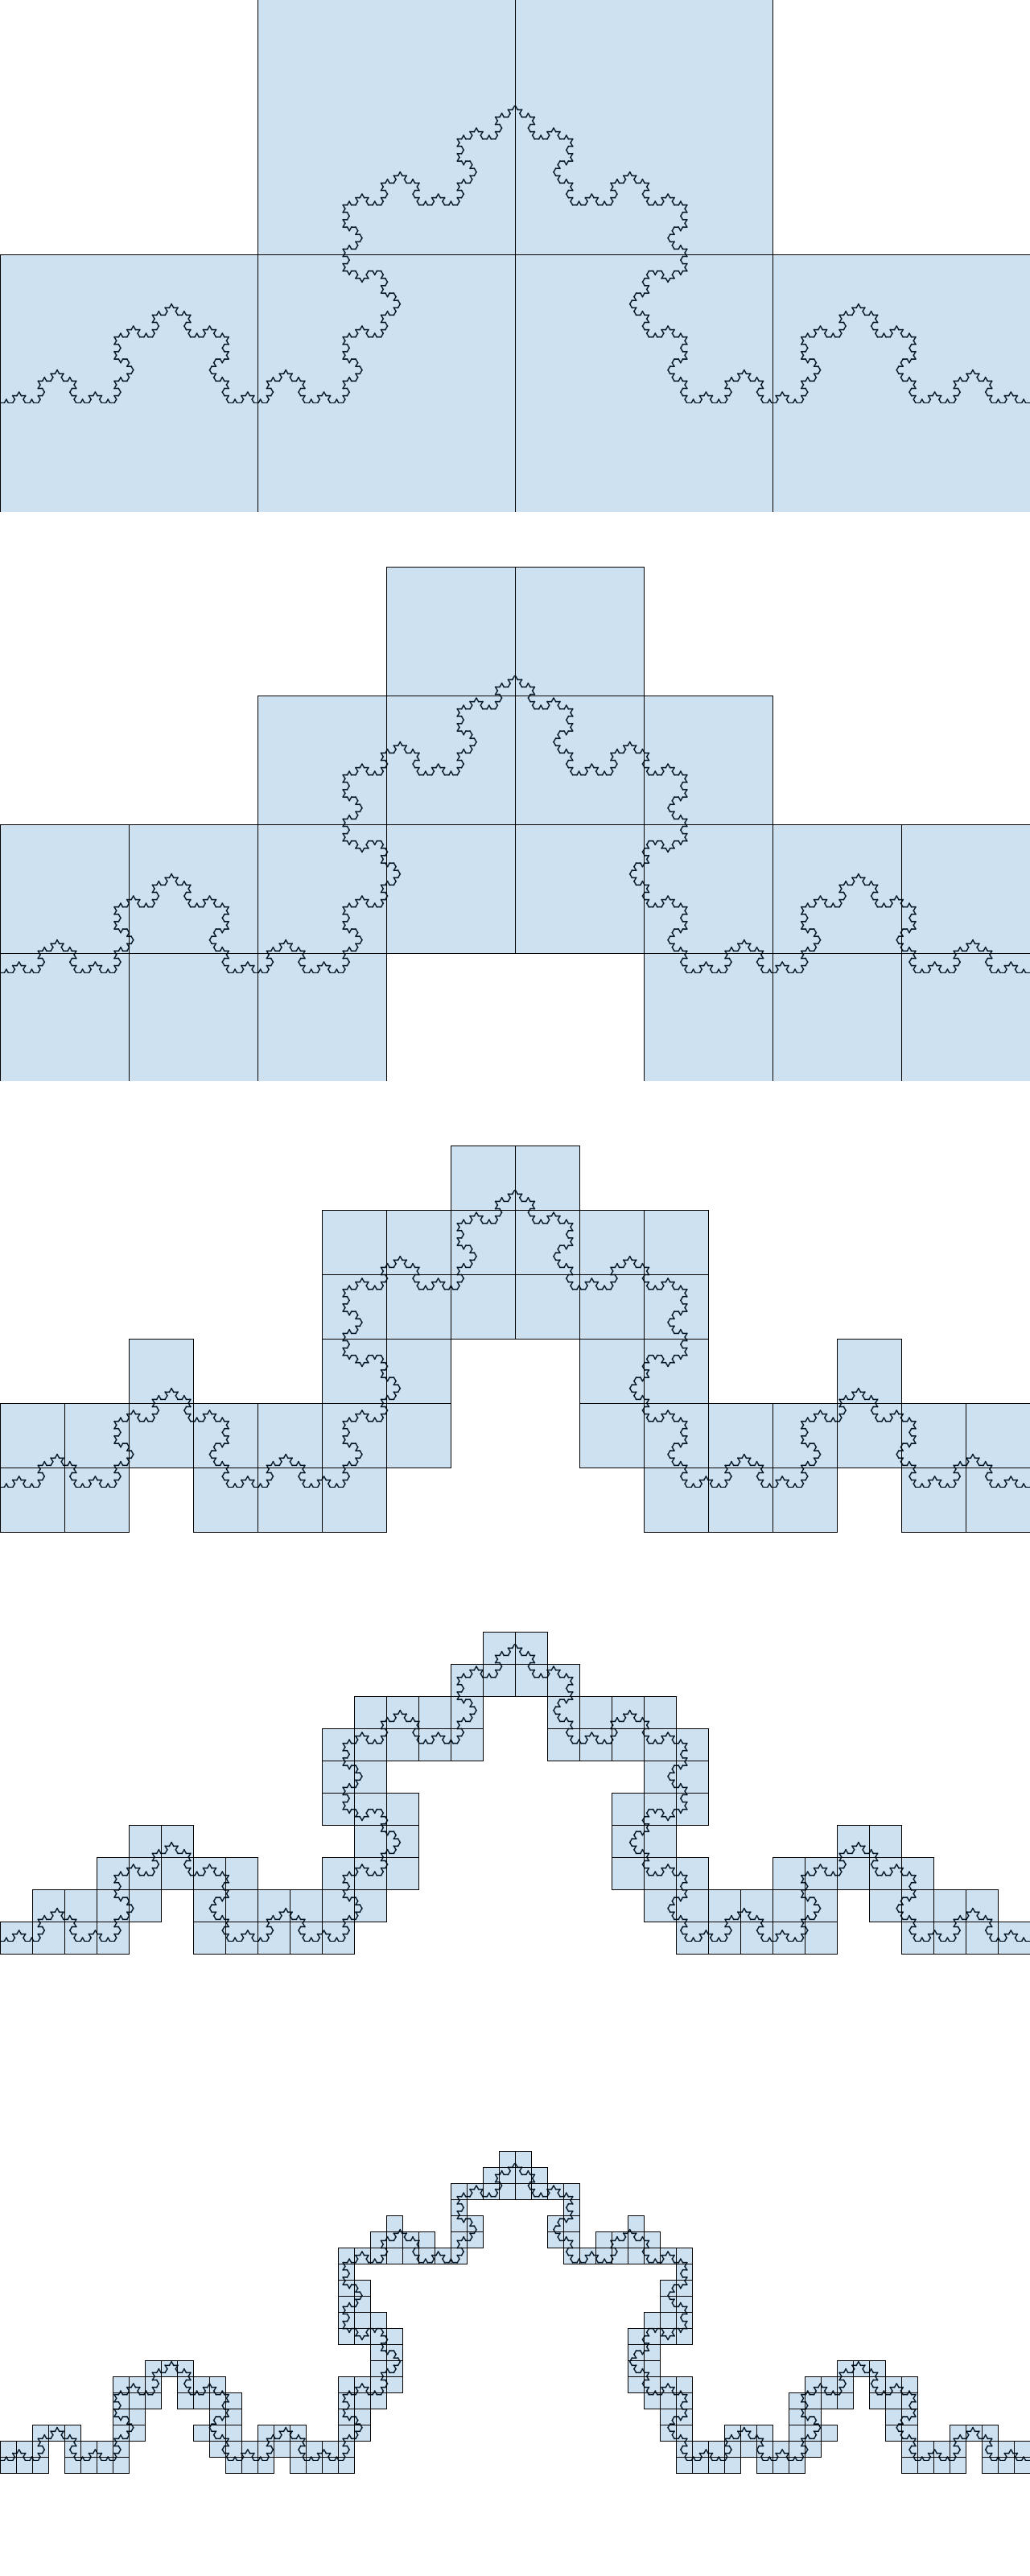
\includegraphics[width=0.5\textwidth]{figures/box-counting-koch-snowflake.png}
    \caption{Box counting del copo de Koch.}
    \label{fig:box-counting-koch-snowflake}
\end{figure}

\begin{theorem}
    El copo de Kock tiene longitud infinita, pero área finita. \cite{youtube-2022}
\end{theorem}

\begin{proof}
    \noindent Primero definamos $N(n)$ como el número de lados del polígono en la iteración $n$ y $L(n)$ como la longitud de cada lado del polígono en la iteración $n$.\\

    \noindent En el inicio, $N(0) = 3$ y $L(0) = 3$\\
    
    \begin{figure}[H]
        \centering
        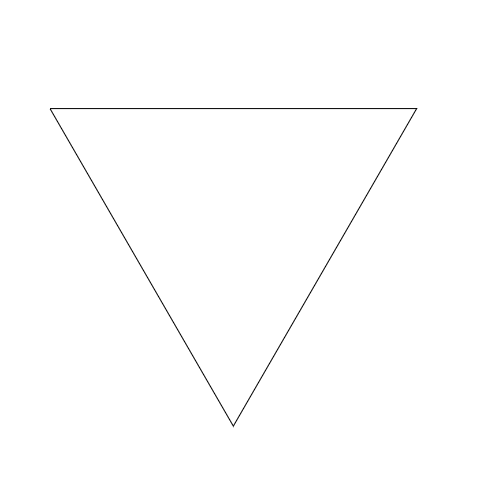
\includegraphics[width=0.5\textwidth]{figures/koch-snowflake-iteration-0.png}
        \caption{Iteración cero del copo de Koch.}
        \label{fig:koch-snowflake-iteration-0}
    \end{figure}
    
    \noindent En la primera iteración, $N(1) = 3 \cdot 4$ y $L(1) = 3 \cdot \frac{4}{3}$\\
    
    \begin{figure}[H]
        \centering
        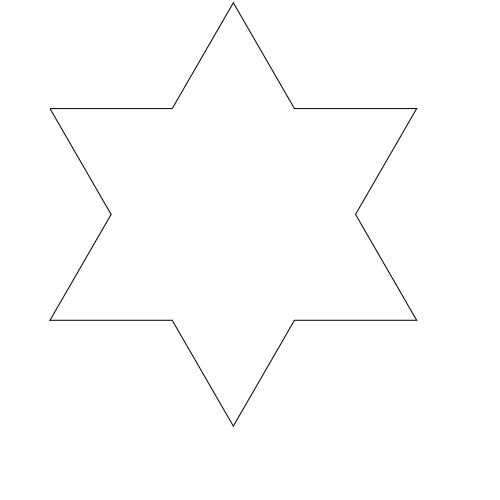
\includegraphics[width=0.5\textwidth]{figures/koch-snowflake-iteration-1.png}
        \caption{Primera iteración del copo de Koch.}
        \label{fig:koch-snowflake-iteration-1}
    \end{figure}
    
    \noindent En la segunda iteración, $N(2) = 3 \cdot 4^2$ y $L(2) = 3 \cdot \left(\frac{4}{3}\right)^2$\\
    
    \begin{figure}[H]
        \centering
        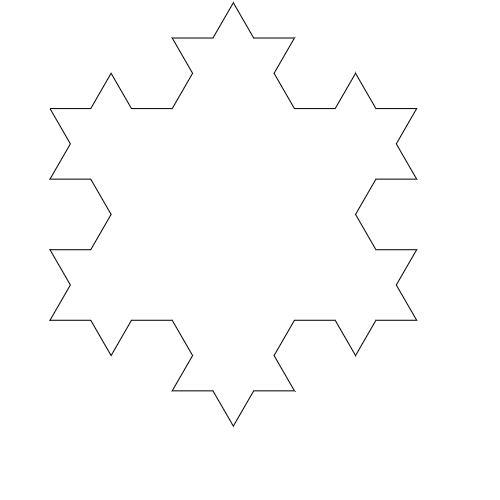
\includegraphics[width=0.5\textwidth]{figures/koch-snowflake-iteration-2.png}
        \caption{Segunda iteración del copo de Koch.}
        \label{fig:koch-snowflake-iteration-2}
    \end{figure}
    
    \noindent En la iteración $n$, $N(n) = 3 \cdot 4^n$ y $L(n) = 3 \cdot \left(\frac{4}{3}\right)^n$\\
    
    \begin{figure}[H]
        \centering
        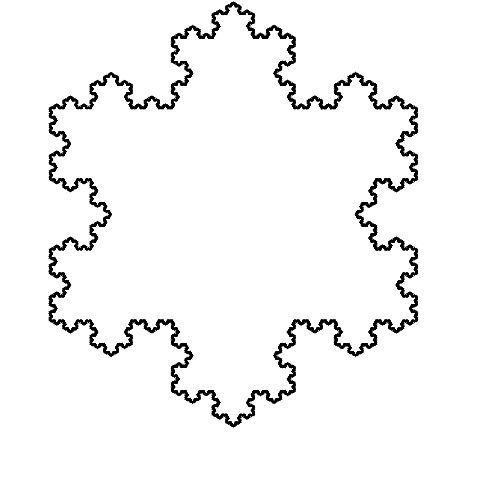
\includegraphics[width=0.5\textwidth]{figures/koch-snowflake-iteration-n.png}
        \caption{Iteración $n$ del copo de Koch.}
        \label{fig:koch-snowflake-iteration-n}
    \end{figure}
    
    \noindent Viendo esto es facil ver que cuando $n \to \infty$, $L(n) \to \infty$\\
    
    \begin{equation}
        \lim_{n \rightarrow \infty}L(n) = \lim_{n \rightarrow \infty} 3 \cdot \left(\frac{4}{3}\right)^n = \infty
    \end{equation}
    
    \noindent El área claramente es finita ya que podemos contener el copo en un círculo. \cite{youtube-2022}\\
    
    \begin{figure}[H]
        \centering
        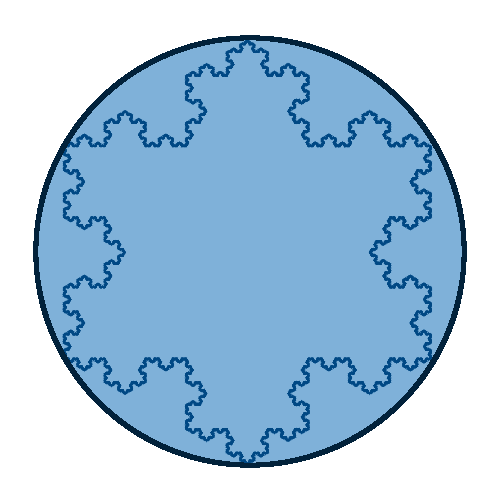
\includegraphics[width=0.5\textwidth]{figures/koch-snowflake-circle.png}
        \caption{Copo de Koch dentro de un círculo.}
        \label{fig:koch-snowflake-circle}
    \end{figure}
\end{proof}

\section{Set de Mandelbrot}

\noindent El set de Mandelbrot es un conjunto bidimensional que con una definición muy simple produce estructuras complejas y hermosas.\\

\noindent Aunque el nombre esté relacionado con el matemático Benoît Mandelbrot, el set fue definido por primera vez en 1978 por Robert W. Brooks y Peter Matelski. \cite{Wikipedia_Mandelbrot}

\begin{figure}[H]
    \centering
    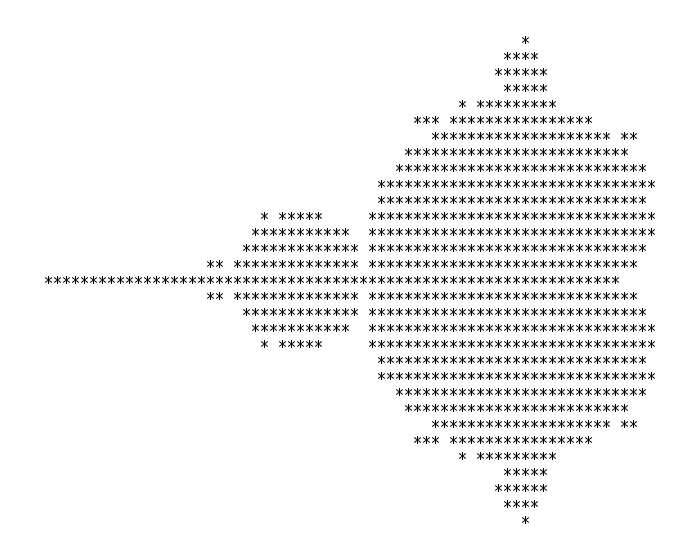
\includegraphics[width=0.5\textwidth]{figures/mandelbrot-set-first-picture.png}
    \caption{Primera imagen publicada del set de Mandelbrot, por Robert W. Brooks y Peter Matelski.}
    \label{fig:mandelbrot-set-first-picture}
\end{figure}

\subsection{Construcción}

\begin{definition}
    El conjunto de Mandelbrot es el conjunto de números complejos $c$ para los cuales el método iterativo definido por $z_0 = 0$ y $z_{n+1} = z_n^2 + c$ no tiende al infinito, es decir, no es divergente.\cite{Medina_2011}
\end{definition}

\noindent En las representaciones gráficas se suele mostrar en negro los puntos que no divergen (los que pertencen al conjunto). El resto de puntos se colorean en función de cuantas iteraciones tardan en exceder un límite en el que ya se supone que divergen.\\

\noindent Para ver si excede el límite podemos usar el módulo del número complejo, el cual representa la distancia de este con el origen. Por ejemplo, si nuestro fractal está definido en $[-1,1] \times [-1,1]$, entonces diremos que $mod(z)>2 \implies \text{divergente}$.
Si completa las $1000$ iteraciones, asumimos que converge y lo pintamos de negro.\\

\begin{lstlisting}[language=Python]
def mandelbrot(x, y):
    c = complex(x, y)
    z = 0

    for i in range(1, 1000):
        if abs(z) > 2:
            return rgb_conv(i)
        z = z * z + c
    return (0, 0, 0)
\end{lstlisting}

\subsection{Propiedades}

\begin{theorem}
    El conjunto de Mandelbrot es compacto. \cite{Wikipedia_Mandelbrot}
\end{theorem}

\begin{lemma}
    Un subconjunto cerrado de un compacto es compacto.
\end{lemma}

\begin{lemma}
    Un círculo es compacto.
\end{lemma}

\begin{lemma}
    El conjunto de Mandelbrot es cerrado.
\end{lemma}

\begin{proof}
    Como el conjunto de Mandelbrot es un conjunto cerrado y es un subconjunto del círculo de radio $2$, entonces también es compacto.
\end{proof}

\begin{theorem}
    El conjunto de Mandelbrot es conexo. \cite{Wikipedia_Mandelbrot}
\end{theorem}

\noindent En 2001, Jeremy Kahn demostró que efectivamente el conjunto es conexo. 

\section{Fractales basados en simulaciones físicas}

\noindent Algunos fractales pueden aparecer como resultado de simulaciones físicas. Esto se debe a que estas simulaciones a menudo producen mucho caos (un pequeño cambio en las condiciones inciales produce resultados dispares), y los fractales están muy relacionados con la teoría del caos.\cite{youtube-2016}\\

\subsection{Fractal a partir de imanes}

\noindent Podemos generar un fractal a partir de tres imanes y una bola de acero colgada de un hilo. Cada pixel representará la posición incial de la bola y el color (rojo, amarillo o azul) representará el imán en el que termina.\\

\begin{figure}[H]
    \centering
    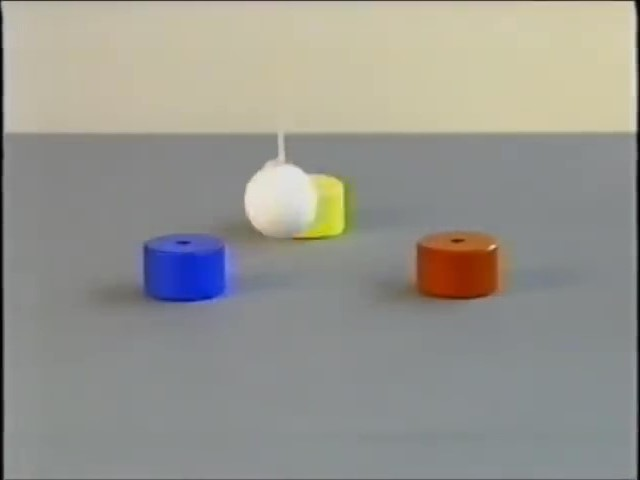
\includegraphics[width=0.5\textwidth]{figures/magnets.jpg}
    \caption{Tres imanes y una bola de acero.}
    \label{fig:magnets}
\end{figure}

\begin{figure}[H]
    \centering
    
\includegraphics[width=0.5\textwidth]{figures/magnet-fractal.jpg}
    \caption{Fractal generado a partir de tres imanes y una bola de acero.}
    \label{fig:magnets-fractal}
\end{figure}

\noindent En cada línea hay otra de diferente color, por lo que podemos seguir haciendo zoom a priori de forma infinita.\\

\begin{figure}[H]
    \centering
    
\includegraphics[width=0.5\textwidth]{figures/magnet-fractal-zoom.jpg}
    \caption{Zoom en el fractal generado a partir de tres imanes y una bola de acero.}
    \label{fig:magnets-fractal-zoom}
\end{figure}

\subsection{Fractal a partir de pelotas rebotando en una función}

\noindent Podemos generar un fractal a partir de una función y una pelota que rebota en ella \cite{balls}. Cada pixel representará la posición incial de la pelota y el color del pixel será cuantos botes tarda en llegar al lado contrario del que empezó. Si la pelota rebota más de $1000$ veces suponemos que se queda en bucle y pintamos el pixel de negro\\ 

\noindent Hemos utilizado la función $f(x)= x^4 - x^2$, pero se podrían usar otras funciones.

\begin{figure}[H]
    \centering
    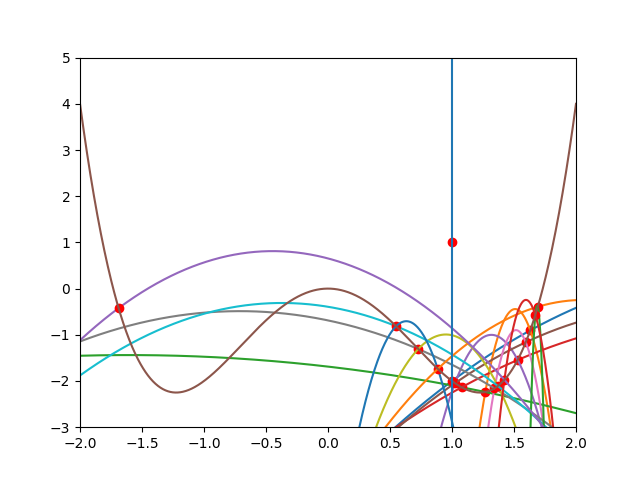
\includegraphics[width=0.7\textwidth]{figures/ball.png}
    \caption{Visualizción de los botes de la pelota $(1,1)$}
    \label{fig:ball-(1,1)}
\end{figure}

\begin{figure}[H]
    \centering
    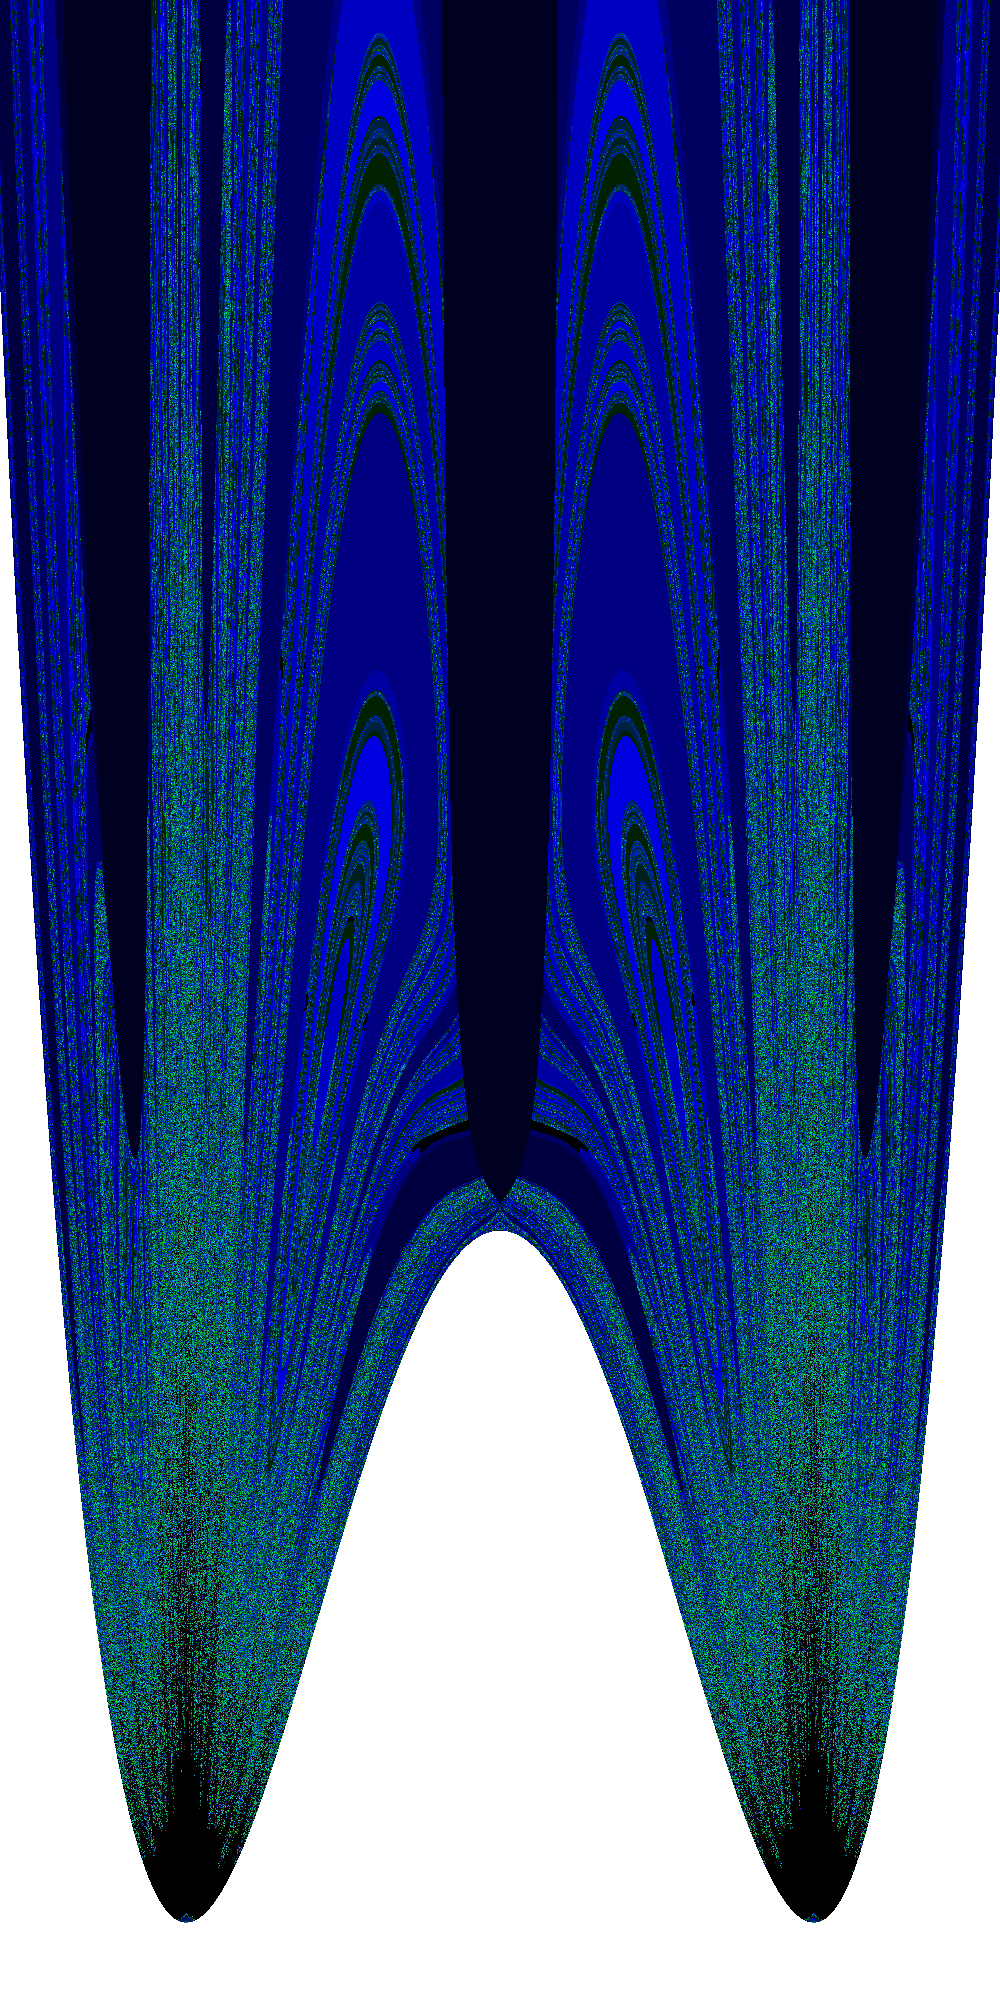
\includegraphics[width=0.7\textwidth]{figures/bouncing-ball-fractal.png}
    \caption{Fractal generado a partir de $f(x) = x^4 - x^2$ y una pelota que rebota en ella.}
    \label{fig:ball-fractal}
\end{figure}

\noindent En las elipses del objeto se puede ver una autosimilitud aproximada. Se parece un poco al fractal magnético.
\begin{figure}[H]
    \centering
    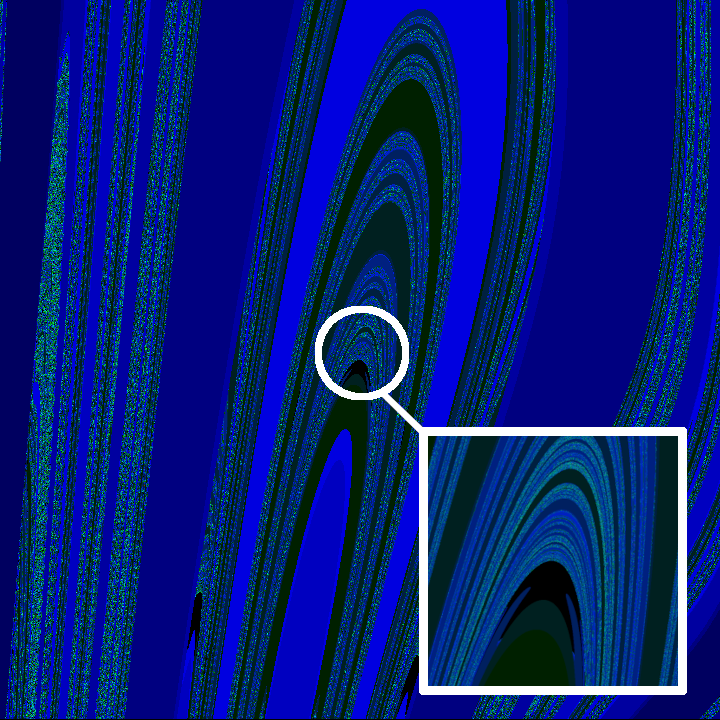
\includegraphics[width=0.7\textwidth]{figures/bouncing-ball-fractal-zoom-1.png}
    \caption{Zoom a una de las elipses del fractal generado a partir de $f(x) = x^4 - x^2$ y una pelota que rebota en ella.}
    \label{fig:ball-fractal-zoom}
\end{figure}

\noindent Hay otras formas interesantes, aunque no tienen autosimilitud.

\begin{figure}[H]
    \centering
    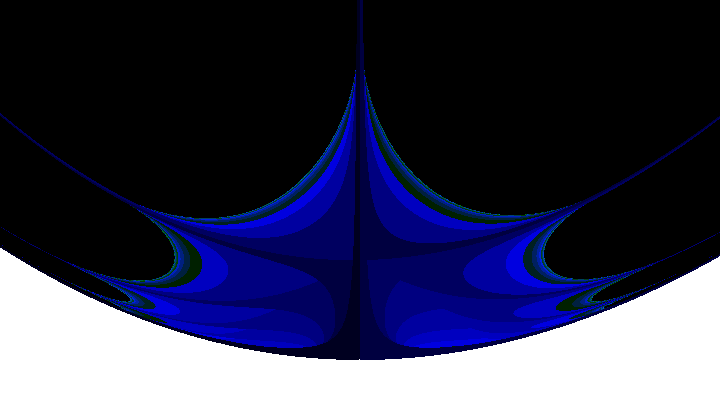
\includegraphics[width=0.7\textwidth]{figures/bouncing-ball-fractal-zoom-2.png}
    \caption{Zoom a una de las patas del fractal generado a partir de $f(x) = x^4 - x^2$ y una pelota que rebota en ella.}
    \label{fig:ball-fractal-zoom-2}
\end{figure}


\chapter{Aplicaciones}

\noindent Se han podido aprovechar los fractales áreas como: Matemáticas, Física, Química, Comunicaciones, Informática, Geología, Economía, Música, Biología, etc…\\

\section{Fractales en la naturaleza}

\noindent Los fractales se pueden encontrar en la naturaleza, por ejemplo, en la forma de las hojas, las ramas de los árboles, las venas de las hojas, las costas, las montañas, los copos de nieve, los relámpagos, los cristales, etc.\\

\noindent Si conseguimos identificar una estructura fractal en un fenómeno natural, podemos estudiar de forma matemática su comportamiento a futuro, permitiendo explicar procesos complejos con fórmulas relativamente simples (como ya vimos en la generación con L-systems)\\

\section{Aplicaciones en la biología}

\noindent Los fractales, además de ser usados en el estudio del crecimiento de las plantas, son usados en:

\begin{itemize}
    \item El estudio de problemas pulmonares, ya que los pulmones presentan una estructura fractal para repartir el aire de forma homogénea.
    
    \begin{figure}[H]
        \centering
        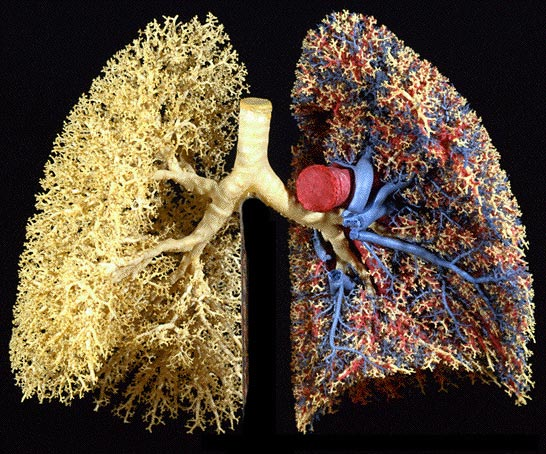
\includegraphics[width=0.5\textwidth]{figures/lungs-fractal.jpg}
        \caption{Estructura fractal de los pulmones.} \cite{BBVA-2020}
        \label{fig:lungs}
    \end{figure}

    \item La evolución de especies depreadoras en entornos controlados pueden representar patrones fractales. \cite{fractales-img}
    
    \item El estudio del ADN y los enlaces entre nucleótidos. \cite{ADN}.
    
    \begin{figure}[H]
        \centering
        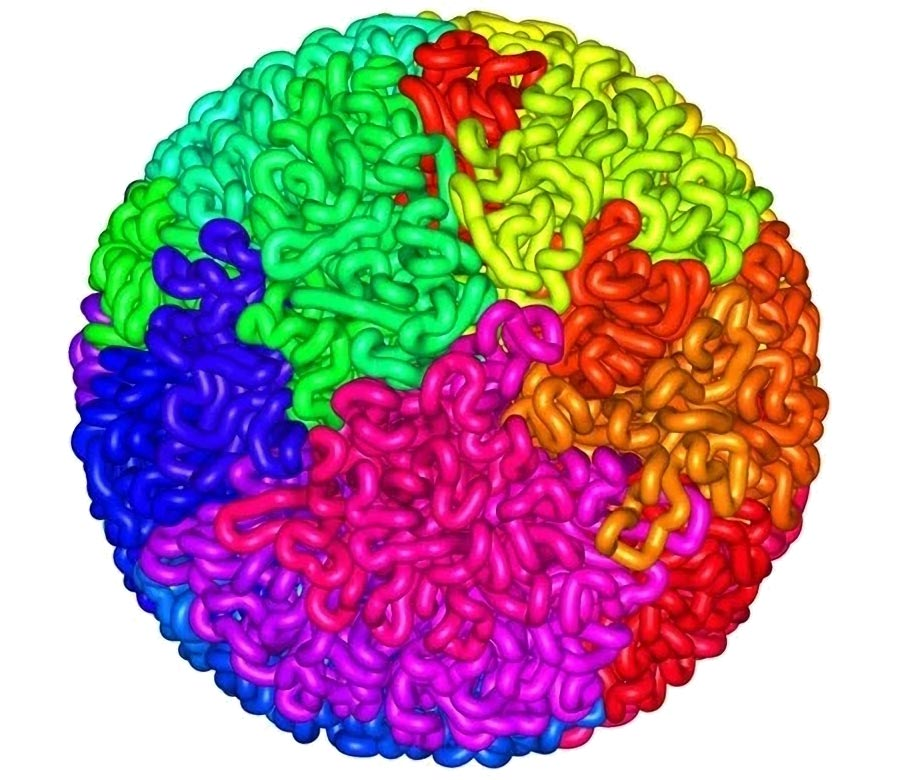
\includegraphics[width=0.5\textwidth]{figures/fractal-genome.jpg}
        \caption{Imagen de como el ADN se compacta en una estructura fractal}
        \label{fig:fractal-genome}
    \end{figure}
\end{itemize}

\section{Aplicaciones en comunicaciones}

\noindent En comunicaciones e informática se experimenta con la compresión fractal de archivos para que ocupen menos espacio.\cite{compresion-fractal} \\

\begin{figure}[H]
    \centering
    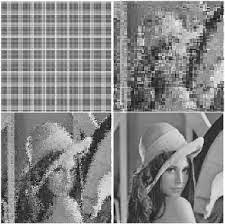
\includegraphics[width=0.5\textwidth]{figures/fractal-compression.jpeg}
    \caption{Ejemplo de compresión fractal}
    \label{fig:fractal-compression}
\end{figure}

\noindent También se ha experimentado con las redes de ordenadores con estructura fractal para comprobar si generan mejor rendimiento. \cite{fractales-img}

\section{Aplicaciones en la geología}

\noindent En la geología, se usan para estudiar las irregularidades de la costa y relieves del terrenos, además de la distribución de las islas y continentes.\cite{BBVA-2020}\\

\begin{figure}[H]
    \centering
    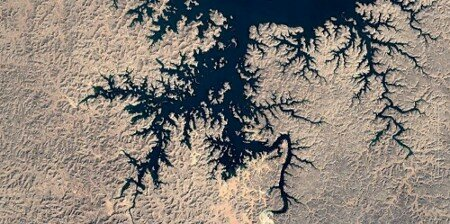
\includegraphics[width=0.5\textwidth]{figures/Lake-Nasser.jpeg}
    \caption{Lago Nasser, Egipto}
    \label{fig:lake-nasser}
\end{figure}

\noindent Los terremotos tienen una relación fractal entre la intensidad del terremoto y la frecuencia del suceso. \cite{geologia}\\

\section{Otras aplicaciones}

\noindent Los fractales también se usan en:

\begin{itemize}
    \item La ecología, para cuantificar los niveles de CO2 que procesan los bosques. \cite{BBVA-2020}
    \item La astrofísica, para estudiar la formación de estrellas.\cite{BBVA-2020}
    \item La economía, para estudiar el comportamiento de la bolsa.\cite{BBVA-2020}
    
    \begin{figure}[H]
        \centering
        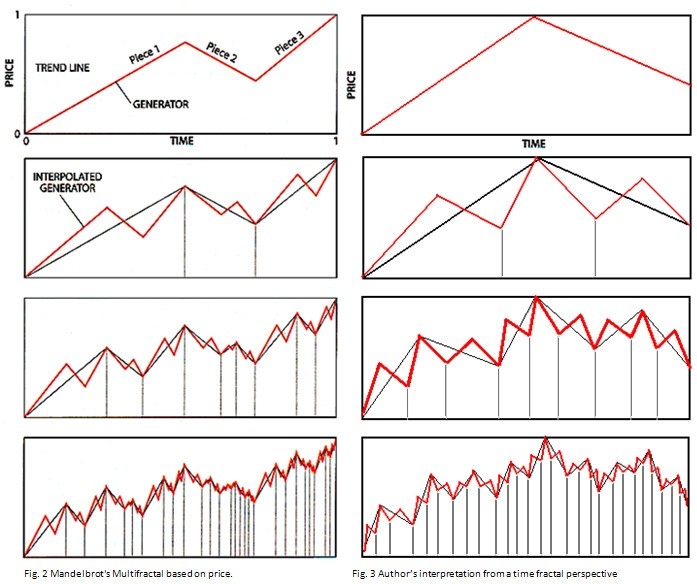
\includegraphics[width=0.5\textwidth]{figures/fractal-economy.jpg}
        \caption{Fractal financiero}
        \label{fig:fractal-economy}
    \end{figure}

    \item Gráficos por ordenador, para generar texturas y paisajes.
    
    \begin{figure}[H]
        \centering
        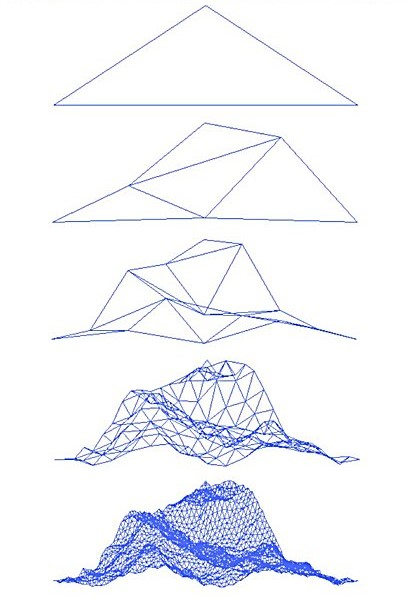
\includegraphics[width=0.5\textwidth]{figures/fractal-mountain.jpg}
        \caption{Fractal que genera una montaña}
        \label{fig:fractal-mountain}
    \end{figure}

\end{itemize}


\appendix

\chapter{Código para la visualización del Box Counting}

\section{Visualización de la recta y el cuadrado}

\begin{lstlisting}[language=Python]
from PIL import Image, ImageDraw

def generar_imagen(n, path):
        
    A = (100,100)
    B = (200,100)
    
    a = (300,100)
    b = (400,100)
    c = (300,200)
    d = (400,200)
        
    img = Image.new('RGB', (500,300), color = 'white')
        
    # Segmento AB
        
    draw = ImageDraw.Draw(img, 'RGBA')
    draw.line((A,B)*100, fill='black', width=1)
        
    # Cuadrado abcd
        
    draw.line((a,b), fill='black', width=1)
    draw.line((b,d), fill='black', width=1)
    draw.line((d,c), fill='black', width=1)
    draw.line((c,a), fill='black', width=1)
    
    # Cajas del segmento AB
    
    for i in range(0,n):
        a = (100+i*(1/n)*100,100+100*1/(2*n))
        b = (100+i*(1/n)*100,100-100*1/(2*n))
        c = (100+(i*100+100)*(1/n),100-100*1/(2*n))
        d = (100+(i*100+100)*(1/n),100+100*1/(2*n))
            
        draw.polygon([a,b,c,d], fill=(0,100,180,50), outline='black', )
        
    # Cajas del cuadrado abcd
        
    for i in range(0,n):
        for k in range(0,n):
            a = (300+k*1/n*100,100+i*1/n*100)
            b = (300+k*1/n*100,100+(i+1)*1/n*100)
            c = (300+(k+1)*1/n*100,100+(i+1)*1/n*100)
            d = (300+(k+1)*1/n*100,100+i*1/n*100)
                
            draw.polygon([a,b,c,d], fill=(0,100,180,50), outline='black')
                
    img.save(path)
        
if __name__ == "__main__":
    N = (2,3,16)
        
    for i in N:
        generar_imagen(i, 'boxcounting-' + str(N.index(i) + 1) + '.png')        
\end{lstlisting}

\section{Visualización del triángulo de Sierpinski}

Créditos a \href{https://github.com/umnikos/Python-Pillow-Library---A-Basic-Example}{umnikos} por el código.

\begin{lstlisting}[language=Python]
from PIL import Image, ImageDraw
import numpy as np
    
size = (512, 512)  # the size of the final image
# create a new black and white image
im = Image.new("1", size, 1)
px = im.load()  # create a pixel access object
    
# takes a 4-tuple range of where to draw the sierpinski triangle
def triangle(xy, fill=0, depth=5):
    # if recursion is over, fill the top left pixel
    if depth == 0:
        px[xy[0], xy[1]] = fill
        return
    # otherwise, draw 3 smaller sierpinski triangles
    triangle(
        (
            (3 * xy[0] + xy[2]) // 4,
            xy[1],
            (xy[0] + 3 * xy[2]) // 4,
            (xy[1] + xy[3]) // 2,
        ),
        fill,
        depth - 1,
    )
    triangle(
        (
            xy[0],
            (xy[1] + xy[3]) // 2,
            (xy[0] + xy[2]) // 2,
            xy[3],
        ),
        fill,
        depth - 1,
    )
    triangle(
        (
            (xy[0] + xy[2]) // 2,
            (xy[1] + xy[3]) // 2,
            xy[2],
            xy[3],
        ),
        fill,
        depth - 1,
    )
    
# draw the triangle (smaller depths results in a dotty output)
triangle((0, 0, size[0], size[1]), depth=10)
            
im.save("sierspinsky.png", "PNG")  # save the image
\end{lstlisting}

\section{Visualización de Box Counting para el triángulo de Sierpinski}

\begin{lstlisting}[language=Python]
import numpy as np
from PIL import Image, ImageDraw

triangle = Image.open('sierspinsky.png')

# Cargar imagen como matriz de pixeles
img_array = np.array(triangle)

def check_pixel_square(top_point, size):
    for i in range(0, size):
        for k in range(0, size):
            if img_array[top_point[1]+ i][top_point[0] + k] == False:
                return True
    return False

def generate_image(n, path):
    img = Image.new('RGB', (512,512), color = 'white')
    img.paste(triangle, (0,0))

    draw = ImageDraw.Draw(img, 'RGBA')

    size = int(512 / n)

    num_cajas = 0

    for i in range(0, n):
        for k in range(0, n):
            if check_pixel_square((i*size,k*size), size):
                draw.rectangle([(i*size,k*size),((i+1)*size,(k+1)*size)], fill=(0,100,180,50), outline='black', width=1)
                num_cajas += 1

    img.save(path)
    print(num_cajas)
    
if __name__ == "__main__":
    
    N = (2,4,8,16)
    
    for i in N:
        generate_image(i, 'boxcounting-sierspinsky-' + str(N.index(i) + 1) + '.png')
\end{lstlisting}

\bibliographystyle{plainurl}
\bibliography{bibliography.bib}


\end{document}